\chapter{Reconstruction and Regression with Binary-Valued Graph Signals} % Main chapter title

\label{chap:binary} 

\lhead{Chapter 7. \emph{Reconstruction and Regression with Binary-Valued Graph Signals}} 

Up to this point in this thesis, our attention has been focused on reconstruction and regression models for real-valued graph signals, as discussed in \cref{chap:gsr_2d,chap:kgr_rnc_2d,chap:nd_gsp,chap:variance}. In this chapter, we shift our attention to scenarios where the signal of interest is binary-valued, which can be employed to describe node classification tasks conducted over networks. For example, consider the task of predicting whether each user in a social network will engage with a specific online advertisement. Assuming it is shown to a subset of the user population, we can represent the outcome (click/no click) as a partially observed binary graph signal across the network. It is reasonable to assume that closely connected users will exhibit a more similar propensity to click than distantly connected users; in other words, we might expect that the click probability varies smoothly with respect to the topology of the graph. Hence, incorporating this relational information into a predictive task could potentially improve its accuracy.

This example represents a binary classification task over the network since there are only two possible outcomes. However, there may also be situations in which each node must be classified into one of $C > 2$ groups. Again, it may be reasonable to assume that the relative class probabilities vary smoothly over the graph. \Cref{fig:binary_class_graph,fig:mutliclass_graph} give visual representations of binary and multiclass classification tasks over a network, respectively.


\begin{figure}[t] 
    \begin{center}
        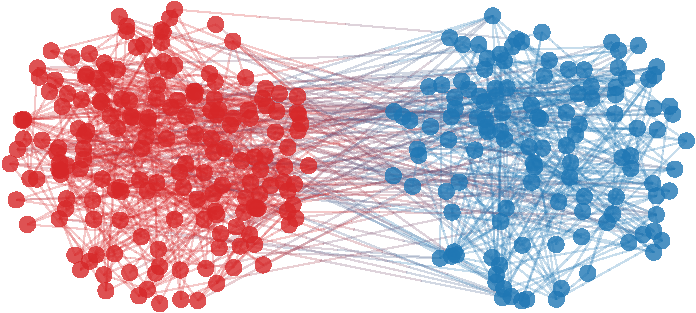
\includegraphics[width=0.7\linewidth]{Figures/2class_graph.pdf}
    \end{center}
   \caption[Visualisation of a binary classification task over a network]{An example visualisation of a binary classification task over a network, with red and blue representing the true binary labels of each node.} 
    \label{fig:binary_class_graph}
\end{figure} 

\begin{figure}[t] 
    \begin{center}
        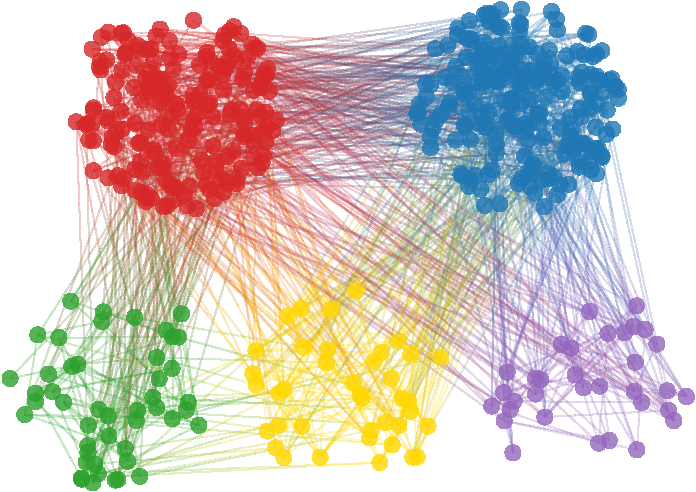
\includegraphics[width=0.7\linewidth]{Figures/multiclass_graph.pdf}
    \end{center}
   \caption[Visualisation of a multiclass classification task over a network]{An example visualisation of a multiclass classification task over a network. Here, the five distinct colours represent the true class label of each node. } 
    \label{fig:mutliclass_graph}
\end{figure} 

Within the graph signal processing community, a significant amount of research has been dedicated to the study of real-valued signals, since they are naturally well-suited to spectral analysis via the GFT and representation in terms of Gaussian random fields. By contrast, binary-valued graph signals, as well as other discrete or non-Gaussian distributions, have received notably less attention. In the machine learning community, binary graph signals have been studied in the context of semi-supervised learning, see for example \cite{Kondor2002,Zhu2003}. However, there, the graph is usually constructed by considering a distance metric in a feature space, and the focus is on maximising the utility of unlabelled data using algorithms such as label propagation (see, for example, \cite{Zhang2017}). The GSP community, by contrast, focuses on statistical processes that occur over intrinsically graph-structured objects using spectral methods. While some work on binary reconstruction and regression from this perspective has occurred (see, for example, \cite{Tran2020}), many of the prominent GSP algorithms and frameworks are yet to be generalised to binary data. In this chapter, we build on some of the models already developed in this thesis (GSR, KGR and RNC) to define associated ``logistic" reconstruction and regression algorithms (L-GSR, L-KGR and L-RNC). These models are targeted towards applications of interest to the GSP community and apply to multiway graph signals in an arbitrary number of dimensions. This means they are particularly suited to multivariate applications such as hyperspectral image processing, graph time series etc.  

This chapter is structured as follows. First, in \cref{sec:lgsr}, we define a model for Logistic Graph Signal Reconstruction (L-GSR) on a Cartesian product graph. Here, we describe how the real-valued multiway GSR framework we developed in \cref{chap:nd_gsp} can be modified to produce a statistical model to describe $d$-dimensional binary graph signals. By making use of the Conjugate Gradient Method (CGM) in conjunction with the Iteratively Reweighted Least Squares (IRLS) algorithm, we demonstrate how to efficiently estimate the underlying class probabilities at each node. Next, in \cref{sec:multiclass}, we adapt this algorithm to accommodate multiclass classification problems. This necessitates the introduction of a new class of Kronecker operator, which appears in the preconditioned coefficient matrix. Using Gerschgorin's circle theorem we can provide guarantees for the CGM convergence by ascertaining an upper bound for its condition number. In \cref{sec:logistic_regression}, adapt the Kernel Graph Regression (KGR) and Regression with Network Cohesion (RNC) models developed in \cref{chap:kgr_rnc_2d}, and adapt them for the task of binary and multiclass node classification, given additional explanatory variables. Finally, in \cref{sec:logistic_rnc_application}, we explore the behaviour of the L-GSR and L-RNC models on an image segmentation task. In particular, we analyse the interpretation of the hyperparameters $\gamma$ and $\beta$ in the context of the logistic models and provide intuition for how these can be set in practice. We also discuss some of the convergence issues associated with the IRLS algorithm and provide practical solutions for mediating them. 


\section{Logistic Graph Signal Reconstruction (L-GSR)}

\label{sec:lgsr}

In this section, we define a model for the reconstruction of binary signals existing on the nodes of a $d$-dimensional Cartesian product graph, which we term Logistic Graph Signal Reconstruction (L-GSR). As before, the graph is characterised by $d$ graph Laplacians $\left\{\LL^{(i)}\right\}_{i=1}^d$, with the total Laplacian given by their Kronecker sum (see \cref{sec:dd_gsp}). The partially observed graph signal, $\Yt$, is an order-$d$ tensor of shape $(N_1, N_2, .., N_d)$, with binary-valued elements representing the two classes. This is accompanied by another binary tensor, $\St$, of the same shape which, as in previous chapters, contains the information about which elements of $\Yt$ were observed by holding ones where successful observations were made and zeros elsewhere. Where no observation was made (i.e. $\St_{\nn} = 0$), the corresponding element $\Yt_{\nn}$ is set to zero by default. The goal is to predict the value of the graph signal at elements where no observation was made using solely the topology of the graph. As such, the input data for this problem can be summarised as follows. 

\begin{equation*}
    \text{input data} = \left\{\; \Yt \in \{0, 1\}^{N_1 \times ... \times N_d}, \;\; \St \in \{0, 1\}^{N_1 \times ... \times N_d} , \;\; \left\{\LL^{(i)} \in \R^{N_i \times N_i}\right\}_{i=1}^d \; \right\}
\end{equation*}

In the following, we assume each observed element of the tensor $\Yt$ follows a Bernoulli distribution, according to some underlying latent probability tensor $\Mt$, which specifies the expected value of the outcome at each node. All other elements of $\Yt$, which were not in the set of observed elements $\mathcal{S}$, are set to zero with probability one. This can be summarised by the following statistical model. 

\begin{equation}
    \label{eq:lgsr_bern} 
    \Yt_\nn \sim  \begin{cases}
        \text{Bern}\left(\Mt_\nn \right) & \text{if} \;\; \nn \in \mathcal{S} \\
        \text{Bern}\left(0\right) & \text{otherwise}
    \end{cases}
\end{equation}


We refer to $\Mt \in [0, 1]^{N_1, ..., N_d}$ as the mean tensor. It has the same shape as $\Yt$ and elements contained within the interval $[0, 1]$ describing the probability that the corresponding entry of $\Yt$ is one. For a given mean tensor, $\Mt$, the probability of observing a binary signal $\Yt$ is given by the following expression. 

\begin{equation}
    \label{eq:lgsr_prob}
    p(\Yt \, | \, \Mt) = \prod_{\nn \in \mathcal{S}} \Mt_\nn^{\Yt_\nn}\left(1 - \Mt_\nn\right)^{1 - \Yt_\nn}
\end{equation}

As such, the log-likelihood of observing a signal $\Yt$, which is simply the natural log of this expression, is given by 

\begin{align}
    \label{eq:lgsr_logprob}
   \log p(\Yt \, | \, \Mt) &= \sum_{\nn} \St_{\nn} \Big( \Yt_{\nn} \log \Mt_{\nn} + (1 - \Yt_{\nn}) \log \left(1 - \Mt_{\nn}\right) \Big) \notag \\
   &= \s^\top \big(\y \circ \log \muu + \left(\one  - \y\right) \circ \log \left(\one - \muu \right)\big) 
\end{align}

where $\s = \vecrm{\St}, \; \y = \vecrm{\Yt}$ and $\muu = \vecrm{\Mt}$. Here, the logarithm function is understood as being applied element-wise.

The goal of our L-GSR model is to estimate the value of the latent probability tensor $\Mt$ given the partially observed binary graph signal $\Yt$. The key assumption that anchors the model to the graph, and avoids underspecification, is that the probability tensor varies smoothly with respect to the topology of the Cartesian product graph. In previous chapters, when working with real-valued signals, this was achieved by setting a Gaussian prior over the latent signal $\Ft$. However, since the elements of $\Mt$ fall within the interval $[0, 1]$, we need a distribution that naturally supports this range. To achieve this, we follow the approach of standard logistic regression (see, for example, \cite{Murphy2012}), by describing the probability in terms of a logistic link function. In particular, we assume that the mean tensor, $\Mt$, is generated by applying the logistic function to a real-valued tensor graph signal $\Ft \in \R^{N_1 \times ... \times N_d}$ as follows. 

\begin{equation}
    \label{eq:logistic_link}
    \Mt(\Ft) = \frac{\one}{\one + \exp(-\Ft)} \quad \Longleftrightarrow \quad \muu(\f) = \frac{\one}{\one + \exp(-\f)}
\end{equation}

Here, the exponential and division should be interpreted as element-wise. Next, we assume that $\f = \vecrm{\Ft}$ is smooth with respect to the topology of the graph by assigning it the following Gaussian prior. 

\begin{equation}
    \label{eq:f_prior_logit}
    \f  \, \sim \, \mathcal{N}\left( \zero, \, \gamma^{-1} \HH^2 \right) 
\end{equation}

As in previous chapters, the covariance matrix $\HH^2$ is the square of a graph filter operator, derived by applying a filter function $g(\cdot)$ to the product graph Laplacian. In particular, 

\begin{equation*}
    \HH = \U \D_\Gt \U^\top
\end{equation*}

where $\U$ is the Kronecker product of each of the eigenvector matrices of the individual factor graph Laplacians, and $\D_\G = \diag{\vecrm{\Gt}}$ is the diagonalised spectral scaling tensor, created by applying an isotropic or anisotropic graph filter to the corresponding eigenvalues (see \cref{sec:dd_gsp,sec:GSP_dd} for details). 

By applying this prior we encode the belief that $\Ft$ is smooth with respect to the topology of the graph, which is then applied by proxy to the mean tensor $\Mt$. In particular, $\muu$ is distributed on $[0, 1]^N$ according to a multivariate logit-normal distribution. Note that this is distinct from the multivariate logistic-normal distribution, which is produced by applying a softmax function to a random Gaussian vector to produce vectors on a simplex \citep{Atchinson1980}. \Cref{fig:logistic_gsr} gives some visual intuition for this by showing a colourmap of several smooth signals on a 2D lattice graph, along with the corresponding mean tensor $\Mt$. As visible, the qualitative smoothness properties of $\Ft$ broadly translate under the transformation of the logistic link function. That is, increasingly smooth real-valued signals correspond to increasingly smooth signals on the unit interval. 

\begin{figure}[t] 
    \begin{center}
        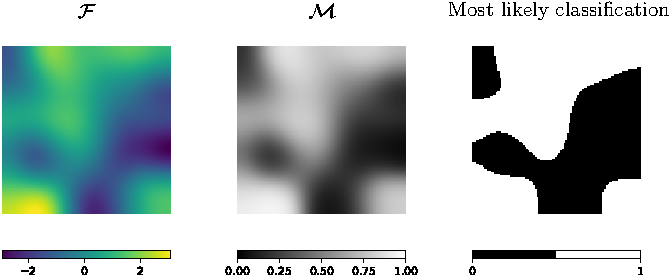
\includegraphics[width=0.9
        \linewidth]{Figures/logistic_gsr.pdf}
    \end{center}
    \caption[Visualisation of binary classification on a 2D lattice]{An example visualisation of transforming a smooth signal via the logistic link function, on a $100 \times 100$ grid of pixels ($N_1 = 100, N_2 = 100$). Left: a random smooth graph signal $\Ft$ drawn from the distribution of \cref{eq:f_prior_logit} with a diffusion filter. Middle: the value of the tensor $\Mt$ found by applying the logistic link function of \cref{eq:logistic_link}. Right: the resultant most likely classification given by $\Mt_{\nn} > 0.5$ each pixel, $\nn$. Each row shows an increasingly smooth signal by increasing the value of $\beta$ characterising the graph filter. } 
    \label{fig:logistic_gsr}
\end{figure} 

As previously stated, the goal of the L-GSR model is to find the most likely value of $\Mt$ given $\Yt$. Since we have a prior distribution over $\Ft$, we can derive an equation for its posterior distribution given $\Yt$ through the application of Bayes' rule. The Maximum A Posteriori (MAP) estimator for $\Ft$ corresponds to the value that minimises the negative log-likelihood of $\Ft \, | \, \Yt$. Given the MAP estimator for $\Ft$, we can compute the most likely mean tensor $\Mt$ by applying \cref{eq:logistic_link}. To this end, we define the objective function $\xi(\f)$, which is equal to $-\log p(\f \, | \, \y)$ up to an additive constant.
 
\begin{equation}
    \label{eq:nll_logistic}
    \xi(\f) = -\s^\top \big(\y \circ \log \muu(\f) + \left(\one  - \y\right) \circ \log \left(\one - \muu(\f) \right)\big) + \frac{\gamma}{2} \f^\top \HH^{-2} \f
\end{equation}

The goal of the next section is to find an algorithm for minimising this expression with respect to $\f$, i.e. to find the MAP estimator for $\Ft$, and subsequently compute the most likely value of the mean tensor $\Mt$. 


\subsection{Solving for the MAP estimator with the IRLS algorithm}

Unlike the normal models of the previous sections, no closed-form solution exists to minimise \cref{eq:nll_logistic}, meaning we must resort to numerical methods. One standard approach is the Iteratively Reweighted Least Squares (IRLS) algorithm. The IRLS algorithm is a numerical method used to solve certain non-linear optimisation problems. It essentially works by iteratively solving a sequence of weighted least squares sub-problems until a satisfactory solution is found. As we will show, in our case, this is particularly attractive, since it is possible to leverage the properties of the Kronecker product to solve these simpler sub-problems efficiently. 

In the context of maximum likelihood estimation for generalised linear models, the IRLS algorithm is equivalent to Fisher's scoring algorithm, which is a variant of the Newton-Raphson method \citep{Nelder1972}. Instead of using the actual Hessian matrix (second derivative of the log-likelihood), Fisher's scoring algorithm uses its expected value, called the Fisher Information matrix. In this setting, each iteration of the IRLS algorithm involves re-weighting the data based on the current estimate of the parameters, then solving a weighted least squares problem to update the parameters, akin to the update step in Fisher Scoring \citep{Fan2020}.

Fisher's scoring algorithm begins with an initial estimate $\f_0$, which is then iteratively refined to reach the global minimum according to the following formula. 

\begin{equation}
    \label{eq:irls_update}
    \f_{k+1} = \f_{k} - \PP^{-1}(\f_k) \, \g(\f_k)
\end{equation}

where $ \g(\f) \in \R^N$ is the gradient of the optimisation objective $\xi(\f)$ with respect to the vector $\f$, and $\PP(\f) \in \R^{N \times N}$ is the Hessian, which is the matrix of second derivatives. 

\begin{equation*}
    \g_n = \frac{\partial \xi(\f)}{\partial \f_n}, \aand \PP_{nm} = \frac{\partial^2 \xi(\f)}{\partial \f_n \partial \f_m}
\end{equation*}

In our case, the gradient is given by 

\begin{equation}
    \g(\f) = \D_\St \big(\muu(\f) - \y\big) + \gamma \HH^{-2} \f
\end{equation}

and the Hessian is given by 

\begin{equation}
    \label{eq:logistic_gsr_P}
    \PP(\f) = \frac{\partial \g(\f)}{\partial \f} =  \D_{\muu}(\f) + \gamma \HH^{-2}
\end{equation}

where $\D_{\muu}(\f)$ is a diagonal matrix with the following definition. 

\begin{equation}
    \D_{\muu}(\f) = \text{diag}\big(\s \circ \muu(\f) \circ (\one - \muu(\f))\big)
\end{equation}

A derivation of the expressions for both the gradient and the Hessian in this context can be found in \cref{the:gradient_and_hesian}. Note that they are both evaluated at a given $\f$. 

Consider the update formula given in \cref{eq:irls_update}. Substituting in the derived values of $\g(\f)$ and $\PP(\f)$, and using the shorthands

\begin{equation*}
    \PP(\f_k) = \PP_k, \quad \g(\f_k) = \g_k, \quad \muu(\f_k) = \muu_k, \aand \D_{\muu}(\f_k) = \D_{\muu}^k
\end{equation*}

gives

\begin{align*}
    \f_{k+1} &= \f_k - \PP^{-1}_k \, \g_k\\
    &= \f_{k} - \PP^{-1}_k \left(\D_\St \big(\muu_k - \y\big) + \gamma \HH^{-2} \f_k\right) \\
    &= \f_k + \PP^{-1}_k \D_\St \big(\y - \muu_k\big) - \PP^{-1}_k (\gamma \HH^{-2} \f_k) \\
    &= \PP^{-1}_k \D_\St \big(\y - \muu_k \big) + \PP^{-1}_k \left(\PP_k \f_k - \gamma \HH^{-2} \f_k\right) \\
    &= \PP^{-1}_k \D_\St \big(\y - \muu_k \big) + \PP^{-1}_k \D_{\muu}^k\f_k  \\
    &= \PP^{-1}_k \left(\D_\St \big(\y - \muu_k \big) + \D_{\muu}^k\f_k \right) \\
    &= \PP^{-1}_k \tee_k
\end{align*}

where

\begin{equation}
    \tee_k = \D_\St \big(\y - \muu_k\big) + \D_{\muu}^k \f_k
\end{equation}

As visible, each iteration of the IRLS algorithm reduces to solving the linear system $\PP^{-1}_k \tee_k$, for some vector $\tee_k$. As such, we must be able to compute a solution to this problem in a maximally efficient way. 


\subsection{Completing IRLS iterations with the CGM}

When it comes to solving the linear system $\PP^{-1}_k \tee_k$, we encounter familiar challenges relating to dimensionality and conditioning. Specifically, the implicit size of $\PP_k$ can be substantial for tensor-valued graph signals, and the inverse-squared filter matrix $\HH^{-2}$ appearing in the definition of $\PP_k$ [see \cref{eq:logistic_gsr_P}] may suffer from severe ill-conditioning. In a similar manner to previous chapters, these issues can be overcome by employing the SIM or CGM techniques introduced in \cref{sec:SIM,sec:CGM}.

In this chapter, our focus will be on the CGM for two primary reasons. Firstly, as the dimensionality of tensor-valued binary graph signals increases, it is likely that only a small fraction of nodes will have valid observed data in most practical applications. As demonstrated in \cref{sec:GSR_convergence_implications}, the CGM exhibits superior scaling properties when the input graph signal $\Yt$ is sparsely observed. Secondly, as discussed in \cref{sec:RNC_solving}, the CGM is applicable to GSR, KGR and RNC problems while the SIM is not suitable for RNC models. Therefore, for simplicity, and for the sake of brevity we focus on the CGM. 

Recall that the CGM seeks to solve a linear system by introducing the symmetric preconditioner $\PSI$, to reduce the condition number of the coefficient matrix. In the case of logistic GSR, we can obtain an alternative expression for the update formula with a reduced condition number as follows. 

\begin{equation*}
    \f_k = \PP^{-1}_k \tee_k \quad \Longrightarrow \quad \f_k = \PSI \Q_k^{-1} \PSI^\top \tee_k
\end{equation*}

where, as in the case of standard real-valued GSR, 

\begin{equation*}
    \PSI = \U \D_\Gt
\end{equation*}

By instead solving the linear system $\Q_k^{-1} (\PSI^\top \tee_k)$ using the conjugate gradient method, and then left-multiplying the result by $\PSI$, we can obtain $\f_{k+1}$ with typically far fewer iterative steps than solving $\PP^{-1} \tee_k$ directly. In this case, $\Q_k$ is given by the following expression. 

\begin{equation}
    \label{eq:Q_LGSR}
    \Q_k = \D_\Gt \U^\top \D_{\muu}^k \U \D_\Gt + \gamma \I_N
\end{equation}

Note that this is similar to the preconditioned coefficient matrix appearing in standard GSR, with the modification that $\D_\St$ has been replaced by $\D_{\muu}^k$. 

The conditioning of the new coefficient matrix $\Q_k$ is significantly improved from the original problem. While the condition number, $\kappa$, of $\PP_k$ was potentially unbounded, $\kappa(\Q_k)$ is guaranteed to have a maximum value of $(0.25 + \gamma) / \gamma$.  This is shown formally in \cref{the:L_GSR_Q_conditioning}. 

\begin{theorem}
    \label{the:L_GSR_Q_conditioning}
    
    The condition number, $\kappa$, of the preconditioned coefficient matrix $\Q_k$, defined in \cref{eq:Q_LGSR}, is bounded as follows. 
    
    \begin{equation}
        \kappa(\Q_k) \leq \frac{0.25 + \gamma}{\gamma}
    \end{equation}

\end{theorem}

\begin{proof}
    As established in \cref{sec:wfl_derivation}, the worst-case convergence rate is achieved in the limit of a weak filter, where $\D_\Gt = \I_N$. In this case, the condition number of $\Q_k$ is given by 

    \begin{align*}
        \kappa(\Q_k) &= \kappa\left( \U^\top \D_{\muu}^k \U + \gamma \I_N\right) \\[0.1cm]
        &=  \kappa\left( \U^\top \left(\D_{\muu}^k + \gamma \I_N\right) \U  \right) \\[0.1cm]
        &= \kappa\left( \D_{\muu}^k + \gamma \I_N\right)
    \end{align*}

    Since $\D_{\muu}^k = \text{diag}\big(\s \circ \muu_k \circ (\one - \muu_k)\big)$, the maximum possible value along the diagonal of $\D_{\muu}^k$ will be 0.25, occurring when the corresponding element of $\muu_k$ is $1/2$. Furthermore, since $\s$ is a binary vector, the smallest possible value along the diagonal is 0. Therefore, the ratio between the largest and smallest eigenvalues of $ \D_{\muu}^k + \gamma \I_N$ must be less than or equal to $(0.25 + \gamma) / \gamma$. 
\end{proof}


\begin{algorithm}[ht]
    \begin{algorithmic}
    \vspace{0.15cm}
    \Require{Observed binary tensor $\Yt \in \{0, 1\}^{N_1 \times ... \times N_d}$}
    \vspace{0.05cm}
    \Require{Binary sensing tensor $\St \in \{0, 1\}^{N_1 \times ... \times N_d}$}
    \vspace{0.05cm}
    \Require{Cartesian product graph Laplacians $\left\{\LL^{(i)} \in \R^{N_i \times N_i}\right\}_{i=1}^d$}
    \vspace{0.05cm}
    \Require{Regularisation parameter $\gamma \in \R^+$}
    \vspace{0.05cm}
    \Require{Graph filter function $g(\, \cdot\, \,; \betaa)$}
    \vspace{0.25cm}
    \State{$\y \leftarrow \vecrm{\Yt}$ }
    \vspace{0.15cm}
    \State{$\s \leftarrow \vecrm{\St}$ }
    \vspace{0.15cm}
    \State{Decompose each $\LL^{(i)}$ into $\U^{(i)} \LAM^{(i)} \left(\U^{(i)}\right)^\top$ }
    \vspace{0.15cm}
    \State{$\U \leftarrow \bigotimes \U^{(i)}$ }
    \vspace{0.15cm}
    \State{Compute $\Gt \in \R^{N_1 \times ... \times N_d}\;$ as $\;\Gt_{\nn} = g\big(\lambdaa(\nn); \, \betaa\big) \quad$ (see \cref{eq:Gn_dd2,eq:lam_of_n})}
    \vspace{0.15cm}
    \State{$\D_\Gt \leftarrow \diag{\vecrm{\Gt}}$}
    \vspace{0.15cm}
    \State{$\D_\St \leftarrow \diag{\s}$}
    \vspace{0.15cm}
    \State{$\PSI \leftarrow \U \D_\Gt$}
    \vspace{0.15cm}
    \State{Initialise $\f \in \R^N$ randomly}
    \vspace{0.25cm}
    \While{$|\Delta \f| > \text{tol}$}
    \vspace{0.15cm}
    \State{$\muu \leftarrow \one / \big(\one + \exp(-\f)\big)$}
    \vspace{0.15cm}
    \State{$\D_{\muu} \leftarrow  \Diag{\vecrm{\s \circ \muu \circ (1 - \muu)}}$}
    \vspace{0.15cm}
    \State{$\tee \leftarrow \D_\St \big(\y - \muu\big) + \D_{\muu} \f $}
    \vspace{0.15cm}
    \State{$\Q \leftarrow  \D_\Gt \U^\top \D_{\muu} \U \D_\Gt + \gamma \I_N$}
    \vspace{0.15cm}
    \State{$\f \leftarrow \PSI \Q^{-1} \PSI^\top \tee \quad$ (solve with the CGM, leveraging the structure of $\Q$)}
    \vspace{0.15cm}
    \EndWhile
    \vspace{0.25cm}
    \State{$\muu \leftarrow \one / \big(\one + \exp(-\f)\big)$ }
    \vspace{0.15cm}
    \Ensure{$\text{reshape} \big( \muu, \, (N_1, ... N_d) \big)$}
    \end{algorithmic}
    \caption{Logistic Graph Signal Reconstruction}
    \label{al:LGSR}
\end{algorithm}

For completeness, we now give the full algorithm for logistic graph signal reconstruction in \cref{al:LGSR}. Note that, by making use of the fast Kronecker product algorithm described in \cref{sec:GSP_dd}, the runtime complexity of the CGM step is bounded by 

\begin{equation*}
    O\left(\frac{0.25 + \gamma}{\gamma} N \sum_{i=1}^d N_i \right)
\end{equation*}

The run time complexity of the overall algorithm of course depends on the convergence rate of the IRLS iterations. This is known to be super-linear, and approximately quadratic when a sufficiently accurate starting value is used \citep{Burden2010}. Whilst an in-depth theoretical exploration of the IRLS algorithm for this particular application is beyond the scope of this chapter, in practice, the IRLS algorithm converges very quickly, usually taking on the order of 10 steps to achieve negligible error.

\section{Multiclass Logistic Graph Signal Reconstruction}

\label{sec:multiclass}

So far we have been focused on binary-valued graph signals, which can be used to represent two-class classification tasks over a multiway network. However, in many practical applications, the task may involve classifying each node into one of multiple distinct groups. Therefore, the objective of this section is to extend and generalise the methods we have developed thus far to encompass multiclass classification problems.

Consider the task of multiclass graph signal reconstruction. Here, the goal is to estimate the probability that each node, $\nn$, in a $d$-dimensional Cartesian product graph belongs to each of $C>2$ distinct classes. To do this, we have access to the factor graph Laplacians $\left\{\LL^{(i)} \in \R^{N_i \times N_i}\right\}_{i=1}^d$, and the true class label at a subset of nodes, $\mathcal{S}$. The partially observed class labels can be represented as an order-($d + 1$) tensor graph signal, where the final dimension contains a ``one-hot" encoding of the class label. As such, the input data for multiclass L-GSR can be summarised as follows. 

\begin{equation*}
    \text{input data} = \Big\{\; \Yt \in \{0, 1\}^{N_1 \times ... \times N_d \times C}, \;\; \St \in \{0, 1\}^{N_1 \times ... \times N_d} , \;\; \left\{\LL^{(i)} \in \R^{N_i \times N_i}\right\}_{i=1}^d\; \Big\}
\end{equation*}

As in previous sections, the tensor $\St$, of shape $(N_1 \times ... \times N_d$), indicates which nodes in the product graph have been successfully observed by holding a one in the corresponding entry, and zeros elsewhere. Note that the observed graph signal, $\Yt$, has an additional dummy dimension of length $C$ to represent the class label, which is not present in $\St$. Where no observation was made (i.e. $\St_{\nn} = 0$), all values along the corresponding fibre $\Yt_{\nn, :}$ can be safely set to zero by default. Note that $\Yt_{\nn, :}$ can have a maximum of one non-zero entry. 

We describe the probability that node $\nn$ has class $c$ by introducing another tensor, $\Mt$. Like $\Yt$, this tensor has shape $(N_1 \times ... \times N_d \times C)$. Each fibre $\Mt_{\nn, :}$ is interpreted as the probability mass function over the $C$ mutually exclusive classes at node $\nn$. In particular, 

\begin{equation*}
    p(\text{node} \; \nn \; \text{is of class} \; c) = \Mt_{\nn, c}, \quad \sum_{c=1}^C \Mt_{\nn, c} = 1
\end{equation*}

Since every length-$C$ fibre $\Mt_{\nn, :}$ must sum to one, the tensor $\Mt$ exists in the space of $N$ independent $C$-dimensional simplexes with $C-1$ degrees of freedom. 

This implies that, for a given value of $\Mt$, the probability of observing a signal $\Yt$ is given by

\begin{equation}
    p(\Yt \, | \, \Mt) = \prod_{c, \nn \in \mathcal{S}} \Mt_{\nn, c}^{\Yt_{\nn, c}}
\end{equation}

As such, the log-likelihood of observing a signal $\Yt$, for a given value of $Mt$, is

\begin{align}
    \log p(\Yt \, | \, \Mt) &= \sum_{\nn, c} \St_{\nn} \, \Yt_{\nn, c} \log \Mt_{\nn, c} \notag \\
    &= (\s \otimes \one_C)^\top \big(\y \circ \log \muu \big)
 \end{align}
 

where, as before, $\s = \vecrm{\St}, \; \y = \vecrm{\Yt}$ and $\muu = \vecrm{\Mt}$. Furthermore, to enforce the restriction that all probabilities must sum to one, we can generate $\Mt$ by applying a softmax function to each length-$C$ fibre of a tensor $\Ft$. 

\begin{equation}
    \label{eq:softmax}
    \Mt_{\nn, c} = \frac{\exp(\Ft_{\nn, c})}{ \raisebox{-0.1cm} { $\sum_{c'=1}^C \exp(\Ft_{\nn, c'})$ }}  \quad \Longleftrightarrow \quad \muu(\f) = \frac{\exp(\f)}{ \big((\I_N \otimes \one_C) \exp(\f)\big) \otimes \one_C}
\end{equation}

Here, $\Ft$ is a real-valued tensor signal which, like $\Mt$ and $\Yt$, has shape $(N_1 \times ... \times N_d \times C)$. A graphical representation of the relation between $\Ft$, $\Mt$ and the most likely classification is shown in \cref{fig:logistic_gsr_multiclass}. The goal, then, of multiclass logistic graph signal reconstruction is to find the most likely value for the tensor $\Ft$, which allows us to make a prediction for the probability of each class by applying \cref{eq:softmax}.  

\begin{figure}[t]  
    \begin{center}
        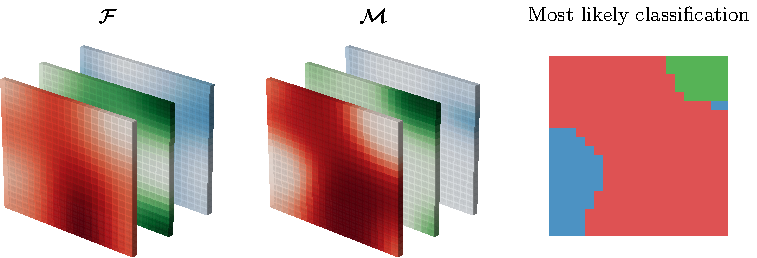
\includegraphics[width=\linewidth]{Figures/multiclass.pdf}
    \end{center}
   \caption[Visualisation of multiclass classification on a 2D lattice]{An example visualisation of transforming a smooth tensor signal via the softmax function on a $20 \times 20$ grid of pixels ($N_1 = 20, N_2 = 20, C=3$). Left: a random smooth tensor signal $\Ft$, drawn from the Gaussian distribution specified in \cref{eq:f_prior_mc_lgsr}, split across three channels. Middle: the value of the tensor $\Mt$ found by applying the softmax function of \cref{eq:softmax} in the class dimension. Right: the resultant most likely classification given by the maximum probability class label for each pixel. } 
    \label{fig:logistic_gsr_multiclass}
\end{figure} 


Assuming no particular relational structure between the $C$ classes, we can encode the assumption that class probabilities should vary smoothly over the graph by assigning the following prior to $\Ft$. 

\begin{equation}
    \label{eq:f_prior_mc_lgsr}
    \f \sim \Norm{\zero}{\gamma^{-1} \HH^2 \otimes \I_C}
\end{equation}

By applying Bayes' rule, we can therefore derive an expression $\xi(\f)$, representing the negative log-likelihood of observing an underlying signal $\f$ given an observed signal $\y$. 

\begin{equation}
    \xi(\f) = - (\s \otimes \one_C)^\top \big(\y \circ \log \muu(\f) \big) + \frac{\gamma}{2} \f^\top \left(\HH^{-2} \otimes \I_C\right) \f
\end{equation}

Once again, we can solve for the minimising value of $\f$ using the IRLS algorithm. In this case, the gradient and Hessian are respectively given by 

\begin{equation}
    \g(\f) = \big(\D_\St \otimes \I_C\big) \big(\muu(\f) - \y\big) + \gamma \left(\HH^{-2} \otimes \I_C\right) \f
\end{equation}

and

\begin{equation}
    \PP(\f) = \RR_{\muu}(\f) + \gamma \HH^{-2} \otimes \I_C
\end{equation}

Unlike the binary model where the Hessian was the sum of a diagonal matrix $\D_{\muu}(\f)$ and $\gamma \HH^{-2}$, the matrix $\RR_{\muu}(\f)$ is no longer diagonal. In this case, $\RR_{\muu}(\f)$ is given by 

\begin{equation}
    \RR_{\muu}(\f) =  \big(\D_\St \otimes \I_C\big) \left(\Diag{\muu(\f)} - \sum_{n=1}^N \mathbf{\Delta}_{n} \otimes \m_n (\f) \m_n^\top(\f) \right)
\end{equation}

where $\m_n \in \R^C$ is the probability mass function at node $n$ (i.e. the $n$-th lexicographically ordered fibre within the tensor $\Mt$), and $\mathbf{\Delta}_{n}$ is a matrix of zeros, with a single one at element $(n, n)$. Given the definition of the Kronecker product, we can see that $\RR_{\muu}(\f)$ is a block-diagonal matrix with the following structure. 

\begin{equation*}
    \RR_{\muu}(\f) = \begin{bmatrix}
        \B_1 & & & \\
        & \B_2 & & \\
        & & \ddots & \\
        & & & \B_N
    \end{bmatrix}, \quad \text{where} \quad \B_n = \s_n \Big(\diag{\m_n} - \m_n \m_n^\top\Big)
\end{equation*}

Despite no longer being diagonal, we can still leverage the block structure of this matrix to multiply $\RR_{\muu}(\f)$ onto an arbitrary vector, $\ve$, efficiently. This can be achieved as follows. 


\begin{equation}
    \label{eq:R_mu_eff}
    \RR_{\muu}(\f) \ve = (\s \otimes \one_C) \circ  \muu(\f) \circ \ve - \Big(\big((\D_\St \otimes \one_C) (\muu(\f) \circ \ve) \big) \otimes \one_C \Big) \circ \muu(\f)
\end{equation}

While a naive implementation of the product $\RR_{\muu}(\f) \ve$ would have memory time and memory complexity $O\left(C^2N^2\right)$, by following the formula given in \cref{eq:R_mu_eff}, it can instead be achieved with time complexity $O(NC^2)$ and memory complexity $O(NC)$. 

Now consider the IRLS update formula. As before, we will use the following shorthands. 

\begin{equation*}
    \PP(\f_k) = \PP_k, \quad \g(\f_k) = \g_k, \quad \muu(\f_k) = \muu_k, \aand \RR_{\muu}(\f_k) = \RR_{\muu}^k
\end{equation*}

Applying the update formula gives

\begin{align*}
    \f_{k+1} &= \f_k - \PP^{-1}_k \, \g_k\\
    &= \f_{k} - \PP^{-1}_k \Big(\big(\D_\St \otimes \I_C\big) \big(\muu_k - \y\big) + \gamma \left(\HH^{-2} \otimes \I_C\right) \f_k\Big) \\
    &= \f_k + \PP^{-1}_k \big(\D_\St \otimes \I_C\big) \big(\y - \muu_k\big) - \PP^{-1}_k \Big(\gamma \left(\HH^{-2} \otimes \I_C\right) \f_k\Big) \\
    &= \PP^{-1}_k \big(\D_\St \otimes \I_C\big) \big(\y - \muu_k \big) + \PP^{-1}_k \Big(\PP_k \f_k - \gamma \left(\HH^{-2} \otimes \I_C\right) \f_k\Big) \\
    &= \PP^{-1}_k \big(\D_\St \otimes \I_C\big) \big(\y - \muu_k \big) + \PP^{-1}_k \RR_{\muu}^k\f_k  \\
    &= \PP^{-1}_k \left(\big(\D_\St \otimes \I_C\big)\big(\y - \muu_k \big) + \RR_{\muu}^k\f_k \right) \\
    &= \PP^{-1}_k \tee_k
\end{align*}

where 

\begin{equation*}
    \tee_k = \big(\D_\St \otimes \I_C\big)\big(\y - \muu_k \big) + \RR_{\muu}^k\f_k
\end{equation*}

As before, we can solve the linear system $\PP^{-1}_k \tee_k$ by introducing a symmetric preconditioner $\PSI$. The only modification is that it must be of dimension $(NC \times NC)$, rather than $(N \times N)$. This can be achieved as follows. 

\begin{equation*}
    \PSI = \left(\U \D_\Gt\right) \otimes \I_C 
\end{equation*}

Using this, we can transform the linear system into 

\begin{equation*}
    \f_k = \PP^{-1}_k \tee_k \quad \Longrightarrow \quad \f_k = \PSI \Q_k^{-1} \PSI^\top \tee_k
\end{equation*}

where 

\begin{equation}
    \label{eq:Q_LGSR_mc}
    \Q_k = \big(\U \D_\Gt \otimes \I_C\big)^\top  \RR_{\muu}^k \big(\U \D_\Gt \otimes \I_C\big) + \gamma \I_{NC}
\end{equation}

Once again, the effect of introducing this preconditioner is to radically improve the conditioning of the coefficient matrix. Again, while the condition number, $\kappa$, of $\PP_k$ is potentially unbounded, $\kappa(\Q_k)$ can be strongly bounded. In particular, it is guaranteed to have a maximum value of $(0.5 + \gamma) / \gamma$. The proof, which is somewhat more involved than the binary case, is given formally in \cref{the:L_GSR_mc_Q_conditioning}. 

\begin{theorem}
    \label{the:L_GSR_mc_Q_conditioning}
    
    The condition number of $\Q_k$ is bounded by a maximum value of 
    
    \begin{equation}
        \kappa(\Q_k) \leq \frac{0.5 + \gamma}{\gamma}
    \end{equation}

\end{theorem}

\begin{proof}
    As established in \cref{sec:wfl_derivation}, the worst-case convergence rate is achieved in the limit of a weak filter, where $\D_\Gt = \I_N$. In this case, the condition number of $\Q_k$ is given by 

    \begin{align*}
        \kappa(\Q_k) &= \kappa\left( \left(\U \otimes \I_C\right)^\top \RR_{\muu}^k \left(\U \otimes \I_C\right) + \gamma \I_{NC}\right) \\[0.1cm]
        &=  \kappa\left( \left(\U \otimes \I_C\right)^\top \left(\RR_{\muu}^k + \gamma \I_N\right) \left(\U \otimes \I_C\right)  \right) \\[0.1cm]
        &= \kappa\left( \RR_{\muu}^k + \gamma \I_N\right)
    \end{align*}

    Since $\RR_{\muu}^k$ is block-diagonal, the set of associated eigenvalues is equal to the union of the eigenvalues of each individual block. Furthermore, each block within  $\RR_{\muu}^k$ is of the form

    \begin{equation*}
        \B = s \Big(\diag{\m} - \m \m^\top\Big)
    \end{equation*}
    
    where $\m \in \R^C$ is a probability mass vector, and $s$ is either zero or one. For the case where $s \neq 0$, we can see that $\B$ must have at least one zero eigenvalue, with eigenvector $\one$, since   

    \begin{align*}
        \B \one &= \Big(\diag{\m} - \m \m^\top\Big) \one \\
        &= \diag{\m} \one - (\m^\top \one) \m \\
        &= \m - \m = \zero
    \end{align*}

    Note, we have used the fact that $\m^\top \one = 1$, since $\m$ represents a probability mass function and must therefore sum to one. Furthermore, we can show that all eigenvalues of $\B$ must be within the interval $[0, 1/2]$, no matter the value of $\m$.  To achieve this, we can make use of the Gerschgorin circle theorem \citep{Gerschgorin1931}. This states that all eigenvalues of a square matrix must fall within at least one of the closed disks $D(a_{ii}, R_i) \subset \mathbb{C}$ in the complex plane. Here, $a_{ii}$ are the centres of the disks given by the diagonal elements of the matrix, and $R_i$ are the radii of the disks, given by 

    \begin{equation*}
        R_i = \sum_{j \neq i} |a_{ij}|
    \end{equation*}
    
    i.e. the sum of the absolute value of the off-diagonal elements in row $i$. Consider the structure of $\B$ when $s \neq 0$. 

    \begin{equation*}
        \B = \diag{\m} - \m \m^\top = \begin{bmatrix}
            m_1 - m_1^2 & -m_1 m_2 & \dots & - m_1 m_C \\
            - m_2 m_1 & m_2 - m_2^2 & \dots & -m_2 m_C \\
            \vdots & \vdots & \ddots & \vdots \\
            -m_C m_1 & -m_C m_2 & \dots &m_C- m_C^2
        \end{bmatrix}
    \end{equation*}
    
    where $m = [m_1, m_2, ..., m_C]$. The disk associated with row $c$ will be given by

    $$
    D\left(m_c - m_c^2, \; \sum_{c' \neq c} |-m_c m_{c'}|\right) = D\Big(m_c\,(1 - m_c), \; m_c\,(1 - m_c)\Big)
    $$
    
    In our particular scenario, the matrix $\B$ is symmetric-real, guaranteeing that its eigenvalues are real. This implies that, instead of complex regions, each of these disks represents a real interval. As such, every eigenvalue is constrained to fall within the interval $m_c\,(1 - m_c) \pm m_c\,(1 - m_c) = \big[0, \, 2 m_c\,(1 - m_c)\big]$. The maximum width of this interval occurs when $m_c = 0.5$, resulting in an interval of $[0, 0.5]$. Consequently, the largest possible eigenvalue of matrix $\B$ is 0.5.

    Finally, since $\RR_{\muu}^k$ is composed of blocks $\B_n$, this means the largest possible eigenvalue of $\RR_{\muu}^k$ is 0.5, and the smallest is zero. Therefore

    \begin{equation*}
        \kappa\left( \RR_{\muu}^k + \gamma \I_N\right) \leq \frac{0.5 + \gamma}{\gamma}
    \end{equation*}

    completing the proof.

\end{proof}

We now present the full algorithm for logistic graph signal reconstruction, which is given in \cref{al:LGSR}. Note that, by making use of the fast Kronecker product algorithm described in \cref{sec:GSP_dd}, the runtime complexity of the CGM step is bounded by 

\begin{equation*}
    O\left(\frac{0.5 + \gamma}{\gamma} NC \Big(C + \sum_{i=1}^d N_i \Big)\right)
\end{equation*}

\begin{algorithm}[ht]
    \begin{algorithmic}
    \vspace{0.15cm}
    \Require{Observed binary tensor $\Yt \in \{0, 1\}^{N_1 \times ... \times N_d \times C}$}
    \vspace{0.05cm}
    \Require{Binary sensing tensor $\St \in \{0, 1\}^{N_1 \times ... \times N_d}$}
    \vspace{0.05cm}
    \Require{Cartesian product graph Laplacians $\left\{\LL^{(i)} \in \R^{N_i \times N_i}\right\}_{i=1}^d$}
    \vspace{0.05cm}
    \Require{Regularisation parameter $\gamma \in \R^+$}
    \vspace{0.05cm}
    \Require{Graph filter function $g(\, \cdot\, \,; \betaa)$}
    \vspace{0.25cm}
    \State{$\y \leftarrow \vecrm{\Yt}$ }
    \vspace{0.15cm}
    \State{$\s \leftarrow \vecrm{\St}$ }
    \vspace{0.15cm}
    \State{Decompose each $\LL^{(i)}$ into $\U^{(i)} \LAM^{(i)} \left(\U^{(i)}\right)^\top$ }
    \vspace{0.15cm}
    \State{$\U \leftarrow \bigotimes \U^{(i)}$ }
    \vspace{0.15cm}
    \State{Compute $\Gt \in \R^{N_1 \times ... \times N_d}\;$ as $\;\Gt_{\nn} = g\big(\lambdaa(\nn); \, \betaa\big) \quad$ (see \cref{eq:Gn_dd2,eq:lam_of_n})}
    \vspace{0.15cm}
    \State{$\D_\Gt \leftarrow \diag{\vecrm{\Gt}}$}
    \vspace{0.15cm}
    \State{$\D_\St \leftarrow \diag{\s}$}
    \vspace{0.15cm}
    \State{$\PSI \leftarrow \U \D_\Gt \otimes \I_C$}
    \vspace{0.15cm}
    \State{Initialise $\f \in \R^{NC}$ randomly}
    \vspace{0.25cm}
    \While{$|\Delta \f| > \text{tol}$}
    \vspace{0.15cm}
    \State{$\muu \leftarrow \exp(\f) / \big((\I_N \otimes \one_C) \exp(\f)\big) \otimes \one_C$}
    \vspace{0.15cm}
    \State{$\M \leftarrow \text{reshape}\big(\muu, (N, C)\big)$}
    \vspace{0.15cm}
    \State{$\RR_{\muu} \leftarrow  \big(\D_\St \otimes \I_C\big) \left(\Diag{\muu} - \sum_{n=1}^N \mathbf{\Delta}_{n} \otimes \m_n \m_n^\top \right)\quad$ ($\m_n$ is the $n$-th row of $\M$)}
    \vspace{0.15cm}
    \State{$\tee \leftarrow \big(\D_\St \otimes \I_C\big)\big(\y - \muu \big) + \RR_{\muu}\f$}
    \vspace{0.15cm}
    \State{$\Q \leftarrow  \big(\U \D_\Gt \otimes \I_C\big)^\top  \RR_{\muu} \big(\U \D_\Gt \otimes \I_C\big) + \gamma \I_{NC}$}
    \vspace{0.15cm}
    \State{$\f \leftarrow \PSI \Q^{-1} \PSI^\top \tee \quad$ (solve with the CGM, leveraging the structure of $\Q$)}
    \vspace{0.15cm}
    \EndWhile
    \vspace{0.25cm}
    \State{$\muu \leftarrow \exp(\f) / \big((\I_N \otimes \one_C) \exp(\f)\big) \otimes \one_C$}
    \vspace{0.15cm}
    \Ensure{$\text{reshape}\big(\muu, (N_1, ..., N_d, C)\big)$}
    \end{algorithmic}
    \caption{Multiclass Logistic Graph Signal Reconstruction}
    \label{al:LGSR_mc}
\end{algorithm}

\section{Logistic Graph Signal Regression} 

\label{sec:logistic_regression}

So far in this chapter, we have developed binary and multiclass multiway graph signal reconstruction algorithms, where no additional data exists to help predict the value of the graph signal at the unlabelled nodes. In this section, we explore several circumstances where explanatory variables are at our disposal and propose models to leverage this information to estimate the underlying class label probabilities.

\subsection{Logistic Kernel Graph Regression (L-KGR)}

\label{sec:lkgr}

The first regression models we consider are binary and multiclass Logistic Kernel Graph Regression (L-KGR). The goal of L-KGR is to predict the underlying class probabilities at the nodes of a sequence of multiway graph signals, given that each signal is paired with an associated vector of explanatory variables. In this respect, it parallels the real-valued KGR model introduced in \cref{sec:kgr_mdp} (and extended to general tensor signals in \cref{sec:kgr_dd}), except here we are concerned with classification rather than real-valued regression. As we will demonstrate, mirroring the pattern of previous sections, the L-KGR model can be interpreted as a relatively straightforward extension of logistic graph signal reconstruction. 

\subsubsection{Binary L-KGR}

First, let us consider binary L-KGR. In this case, we have a sequence of $T$ partially observed binary tensor graph signals, $\Yt_t$, each with a shape of $(N_1, ..., N_d)$. As before, each signal is interpreted as existing on the nodes of a $d$-dimensional Cartesian product graph, with factor graph Laplacians $\left\{\LL^{(i)} \in \R^{N_i \times N_i}\right\}_{i=1}^d$. Where no class outcome was recorded, the relevant element in the signal $\Yt_t$ can default to zero. Furthermore, at each time instant, we have a length-$M$ vector of explanatory variables $\x_t$, which is anticipated to have some non-linear explanatory relation to each $\Yt_t$.

The sequence of partially observed signals can be assembled into a single tensor $\Yt$ of shape $(T, N_1, ..., N_d)$. This is accompanied by a binary sensing tensor, $\St$, of the same shape, which indicates which values were observed and which were absent. The explanation variables can also be aggregated into a single object, in this case, a matrix $\X$ with a shape of $(T, M)$. The goal is to leverage the explanatory variables, in conjunction with the topology of the underlying graph, to estimate the class probability at each node, at each time instant. The relevant input data can therefore be described as follows. 


\begin{multline*}
    \text{input data} = \Bigg\{\;\X \in \R^{T \times M}, \;\; \Yt \in \{0, 1\}^{T \times N_1 \times ... \times N_d}, \;\; \\ 
    \St \in \{0, 1\}^{T \times N_1 \times ... \times N_d} , \;\; \left\{\LL^{(i)} \in \R^{N_i \times N_i}\right\}_{i=1}^d \; \Bigg\}
\end{multline*}

Following the same pattern as the KGR algorithms of previous sections (see \cref{sec:KGR_and_GSR} for details and further explanation), we can conveniently derive a logistic kernel graph regression model by making small modifications to the L-GSR model derived in \cref{sec:lgsr}.  

As with L-GSR, we first assume each element of $\Yt$ is distributed according to a Bernoulli distribution, with a mean given by a latent mean tensor $\Mt$, which has the same shape as $\Yt$ (see \cref{eq:lgsr_bern,eq:lgsr_prob,eq:lgsr_logprob}). However, in this case, we assume that $\Mt$ is smooth with respect to both the topology of the graph, \textit{and} with respect to the feature space. (This is admittedly a somewhat vague statement on its own - see \cref{sec:kgr_mdp} for a more detailed model derivation and \cref{sec:KGR_and_GSR} for further intuition). This belief can be encoded by proxy via a tensor $\Ft$, which is again related to $\Mt$ via the logistic link function of \cref{eq:logistic_link}. We implement these assumptions by establishing the following prior distribution for $\f = \vecrm{\Ft}$.

\begin{equation}
    \f \sim \Norm{\zero}{\gamma \K \otimes \HH^2}
\end{equation}

As before, $\K$ is the $T \times T$ kernel matrix created by applying a symmetric function, such as the Gaussian kernel, $\kappa(\cdot, \cdot)$ to pairs of feature vectors such that $\K_{ij} = \kappa(\x_i, \x_j)$. Next, we compute the eigendecomposition of $\K$ as $\K = \V \LAM_K \V^\top$. Finally, we define the transformed variables $\bar{\U}$ and $\bar{\Gt}$ as follows. 

\begin{equation}
    \label{eq:lkgr_substitution}
    \bar{\U}  = \V \otimes \U, \aand \bar{\Gt}_{t, \nn}  = \Gt_{\nn} \sqrt{\lambda_t^{(K)}}
\end{equation}

where $\lambda_t^{(K)}$ is the $t$-th eigenvalue of $\K$. This implies that 

\begin{equation}
    \K \otimes \HH^2 = \bar{\U} \D_{\bar{\Gt}} \bar{\U}^\top
\end{equation}

where $\D_{\bar{\Gt}} = \diag{\vecrm{\bar{\Gt}}}$. The L-KGR algorithm then follows by modifying \cref{al:LGSR} such that every instance of $\U$ and $\Gt$ is substituted for $\bar{\U}$ and $\bar{\Gt}$ respectively. Note that, as with the KGR models of previous sections, this has an impact on the convergence rate of the CGM step, since the condition number of the preconditioned coefficient matrix $\Q_k$ is increased. As a result, the upper bound on the run time complexity for the whole algorithm is given by 

\begin{equation*}
    O\left(\rho(\K)\frac{0.25 + \gamma}{\gamma} TN \Big(T + \sum_{i=1}^d N_i\Big) \right)  \approx O\left( \frac{0.25 + \gamma}{\gamma} T^2 N \Big(T + \sum_{i=1}^d N_i\Big) \right) 
\end{equation*}

\subsubsection{Multiclass L-KGR}

The same principles can be used to generate a multiclass logistic kernel graph regression algorithm. In this case, the input data is a sequence of $T $ partially observed multiway graph signals, where each observed node has been classified into one of $C > 2$ classes. This can be represented by the binary tensor $\Yt$ with shape $(T \times N_1 \times ... \times N_d \times C)$, where an extra dimension has been added containing a one-hot encoding of the class label. Where no data was recorded, the full length-$C$ fibre at time $t$ and node $\nn$ can be set to zero. As such, the data is described as follows. 

\begin{multline*}
    \text{input data} = \Bigg\{\;\X \in \R^{T \times M}, \;\; \Yt \in \{0, 1\}^{T \times N_1 \times ... \times N_d \times C}, \;\; \\ 
    \St \in \{0, 1\}^{T \times N_1 \times ... \times N_d} , \;\; \left\{\LL^{(i)} \in \R^{N_i \times N_i}\right\}_{i=1}^d \; \Bigg\}
\end{multline*}

Just as with the multiclass L-GSR model derived in \cref{sec:multiclass}, we introduce the tensor $\Mt$, with the same shape as $\Yt$, where each length-$C$ fibre $\Mt_{t, \nn, :}$ describes the probability mass function over the $C$ classes for node $\nn$ at time $t$. As before, $\Mt$ is constructed by applying a softmax function to each fibre of another tensor $\Ft$. 

\begin{equation}
    \label{eq:softmax2}
    \Mt_{t, \nn, c} = \frac{\exp(\Ft_{t, \nn, c})}{ \raisebox{-0.1cm} { $\sum_{c'=1}^C \exp(\Ft_{t, \nn, c'})$ }}  \quad \Longleftrightarrow \quad \muu(\f) = \frac{\exp(\f)}{ \big((\I_{NT} \otimes \one_C) \exp(\f)\big) \otimes \one_C}
\end{equation}

We then place a prior over the signal $\f = \vecrm{\Ft} \in \R^{TNC}$ of

\begin{equation}
    \f \sim \Norm{\zero}{\gamma \K \otimes \HH^2 \otimes \I_C}
\end{equation}

This encodes the belief that each of the $c$ class probabilities should vary smoothly (and independently) with respect to the topology of the graph and the feature space. once again, the full procedure for outputting the tensor $\Mt$ can be achieved by running \cref{al:LGSR_mc} after substituting the variables $\U \rightarrow \bar{\U}$ and $\Gt \rightarrow \bar{\Gt}$, as described in \cref{eq:lkgr_substitution}. Given the effect this substitution has on the preconditioned coefficient matrix $\Q_k$ appearing in each iteration of the IRLS algorithm, it is simple to show that the run time complexity of multiclass L-KGR becomes bounded by the following. 

\begin{equation*}
    O\left(\rho(\K) \frac{0.5 + \gamma}{\gamma} TNC \Big(T + C + \sum_{i=1}^d N_i \Big)\right) \approx O\left(\frac{0.5 + \gamma}{\gamma} T^2NC \Big(T + C + \sum_{i=1}^d N_i \Big)\right)
\end{equation*}


\subsection{Logistic Regression with Network Cohesion (L-RNC)}

\label{sec:lrnc}

In this section, we present models for binary and multiclass Logistic Regression with Network Cohesion (L-RNC). These models are relevant when there is a $d$-dimensional Cartesian product graph, for which a subset of nodes have a known class label. In addition, each node has a length-$M$ vector of explanatory variables. The goal is to utilise both the topology of the graph and the explanatory variables to estimate the class probabilities at the unlabelled nodes. 

\subsubsection{Binary L-RNC}

First, let us consider binary L-RNC. In this scenario, we encounter a partially observed binary multiway graph signal $\Yt$, with shape $(N_1 \times ... \times N_d)$, where a subset of the nodes have been labelled with the true class. As before, $\Yt$ is interpreted as existing on the nodes of a known Cartesian product graph, with factor Laplacians $\left\{\LL^{(i)} \in \R^{N_i \times N_i}\right\}_{i=1}^d$. In addition, each node $\nn$ in the product graph has an associated length-$M$ vector of explanatory variables, collected into the tensor $\Xt$ with shape $(N_1 \times ... \times N_d \times M)$. The goal is to predict the class probabilities at each node $\nn$. Once again, we also have a binary tensor $\St$ describing which nodes have been observed. As such, the data for the binary L-RNC algorithm can be summarised as follows. 

\begin{multline*}
    \text{input data} = \Bigg\{\;\Xt \in \R^{N_1 \times ... \times N_d \times M}, \;\; \Yt \in \{0, 1\}^{N_1 \times ... \times N_d}, \;\; \\ 
    \St \in \{0, 1\}^{N_1 \times ... \times N_d} , \;\; \left\{\LL^{(i)} \in \R^{N_i \times N_i}\right\}_{i=1}^d \; \Bigg\}
\end{multline*}

As with the L-GSR model, we suppose that each observed element of $\Yt$ is a Bernoulli random variable, with the probability of success given by the tensor $\Mt \in [0, 1]^{N_1 \times ... \times N_d}$. However, in the L-RNC model, we assume that the probability at each node is given by the logistic function applied to the sum of an intercept term and a linear combination of the explanatory variables at that node. As with the real-valued RNC model introduced in \cref{sec:rnc_mdp}, the intercept term is flexible and assumed to vary smoothly with respect to the topology of the product graph. Denoting $\muu = \vecrm{\Mt}$, this is summarised by the following expression. 

\begin{equation}
    \muu(\cc, \w) = \frac{\one}{\one + \exp\big(-(\cc + \X \w) \big)}
\end{equation}

Here, $\cc = \vecrm{\Ct}$ is the real-valued vector form of a tensor $\Ct$, which is assumed to vary smoothly with respect to the topology of the multiway graph, $\X$ is the tensor of explanatory variables reshaped into a matrix of dimensions $(N \times M)$ (see \cref{eq:X_RNC_dd}), and $\w \in \R^M$ is the length-$M$ vector of coefficients specifying the contribution of each of the explanatory variables. As in previous sections on RNC, we can stack $\cc$ and $\w$ into a single parameter vector $\thetaa$, such that 

\begin{equation}
    \label{eq:lrnc_logistic}
    \muu(\thetaa) = \frac{\one}{\one + \exp\big(-\big[\I_N \;\; \X \big] \thetaa \big)}
\end{equation}

Furthermore, we can place a prior over $\thetaa$ that encodes the belief that $\Ct$ should be smooth with respect to the topology of the Cartesian product graph, as well as preventing overfitting of $\w$ with an L2 penalty. 

\begin{equation}
    \thetaa \sim \Norm{\zero}{\begin{bmatrix}\gamma^{-1} \HH^2 & \zero \\
    \zero & \lambda^{-1} \I_M \end{bmatrix}}
\end{equation}

As such, the MAP estimator for $\thetaa$ is given by the minimiser of the following expression. 

\begin{equation}
    \label{eq:nll_logistic_rnc}
    \xi(\thetaa) = -\s^\top \big(\y \circ \log \muu(\thetaa) + \left(\one  - \y\right) \circ \log \left(\one - \muu(\thetaa) \right)\big) + \frac{1}{2} \thetaa^\top \begin{bmatrix}\gamma^{1} \HH^{-2} & \zero \\
        \zero & \lambda^{1} \I_M \end{bmatrix}\thetaa
\end{equation}

Proceeding in the same way as L-GSR, we must compute both the gradient, $\widetilde{\g}(\thetaa)$, and the Hessian, $\widetilde{\PP}(\thetaa)$, of this expression with respect to $\thetaa$. These are given by 

\begin{equation}
    \widetilde{\g}(\thetaa) \in \R^{N + M} = \begin{bmatrix}
        \D_\St \\ \X^\top \D_\St
    \end{bmatrix} \big(\muu(\thetaa) - \y\big) + \begin{bmatrix}
        \gamma^{-1} \HH^2 & \zero \\
    \zero & \lambda^{-1} \I_M
    \end{bmatrix} \thetaa
\end{equation}

and 

\begin{equation}
    \widetilde{\PP}(\thetaa)  \in \R^{(N + M) \times (N + M)} = \begin{bmatrix}
        \D_{\muu}(\thetaa) + \gamma \HH^{-2} & \D_{\muu}(\thetaa) \X \\ 
        \X^\top \D_{\muu}(\thetaa)  & \X^\top \D_{\muu}(\thetaa) \X + \lambda \I_M
    \end{bmatrix}
\end{equation}

where, as with L-GSR, $\D_{\muu}$ is the diagonal $N \times N$ matrix given by

\begin{equation}
    \D_{\muu}(\thetaa) = \text{diag}\big(\s \circ \muu(\thetaa) \circ (\one - \muu(\thetaa))\big)
\end{equation}

Then, using the shorthands 

\begin{equation*}
    \widetilde{\PP}(\thetaa_k) = \widetilde{\PP}_k, \quad \widetilde{\g}(\thetaa_k) = \widetilde{\g}_k, \quad \muu(\thetaa_k) = \muu_k, \aand \D_{\muu}(\thetaa_k) = \D_{\muu}^k
\end{equation*}

the IRLS update formula can be derived as follows. 

\begin{align*}
    \thetaa_{k + 1} &= \thetaa_k - \widetilde{\PP}^{-1}_k \, \widetilde{\g}_k \\
    &= \thetaa_k - \widetilde{\PP}^{-1}_k \left( \begin{bmatrix}
        \D_\St \\ \X^\top \D_\St
    \end{bmatrix} \big(\muu_k - \y\big) + \begin{bmatrix}
        \gamma^{-1} \HH^2 & \zero \\
    \zero & \lambda^{-1} \I_M
    \end{bmatrix} \thetaa_k \right)\\
    &= \thetaa_k + \widetilde{\PP}^{-1}_k  \begin{bmatrix}
        \D_\St \\ \X^\top \D_\St
    \end{bmatrix} \big(\y - \muu_k\big) - \widetilde{\PP}^{-1}_k  \begin{bmatrix}
        \gamma^{-1} \HH^2 & \zero \\
    \zero & \lambda^{-1} \I_M
    \end{bmatrix} \thetaa_k \\
    &=  \widetilde{\PP}^{-1}_k  \begin{bmatrix}
        \D_\St \\ \X^\top \D_\St
    \end{bmatrix} \big(\y - \muu_k\big) + \widetilde{\PP}^{-1}_k  \left(\widetilde{\PP}_k \thetaa_k - \begin{bmatrix}
        \gamma^{-1} \HH^2 & \zero \\
    \zero & \lambda^{-1} \I_M
    \end{bmatrix} \thetaa_k \right)\\
    &=  \widetilde{\PP}^{-1}_k  \begin{bmatrix}
        \D_\St \\ \X^\top \D_\St
    \end{bmatrix} \big(\y - \muu_k\big) + \widetilde{\PP}^{-1}_k  \begin{bmatrix}
        \D_{\muu}^k & \D_{\muu}^k \X \\ 
        \X^\top \D_{\muu}^k  & \X^\top \D_{\muu}^k \X
    \end{bmatrix} \thetaa_k \\
    &=  \widetilde{\PP}^{-1}_k  \begin{bmatrix}
        \D_\St \\ \X^\top \D_\St
    \end{bmatrix} \left(\y - \muu_k + \D_{\muu}^k \big[\I_N \;\; \X \big] \thetaa_k \right) \\
    &= \widetilde{\PP}_k^{-1} \widetilde{\tee}_k 
\end{align*}

where 

\begin{equation}
    \widetilde{\tee}_k = \begin{bmatrix}
        \D_\St \\ \X^\top \D_\St
    \end{bmatrix} \left(\y - \muu_k + \D_{\muu}^k \big[\I_N \;\; \X \big] \thetaa_k \right)
\end{equation}

Note that, in the derivation above, we have used the fact that $\D_\St \D_{\muu}^k = \D_{\muu}^k \D_\St = \D_{\muu}^k$. This implies that 

\begin{equation*}
    \begin{bmatrix}
        \D_\St \\ \X^\top \D_\St
    \end{bmatrix} \D_{\muu}^k \big[\I_N \;\; \X \big] =  \begin{bmatrix}
        \D_{\muu}^k & \D_{\muu}^k \X \\ 
        \X^\top \D_{\muu}^k  & \X^\top \D_{\muu}^k \X
    \end{bmatrix}
\end{equation*}

As before, the linear system $\widetilde{\PP}_k^{-1} \widetilde{\tee}_k $ cannot easily be solved in this form due to ill-conditioning. To overcome this issue, we can again use the symmetrically preconditioned CGM. In particular, we can transform the system into 

\begin{equation*}
    \thetaa_k = \widetilde{\PP}^{-1}_k \widetilde{\tee}_k \quad \Longrightarrow \quad \thetaa_k = \widetilde{\PSI}_k \widetilde{\Q}_k^{-1} \widetilde{\PSI}_k^\top \widetilde{\tee}_k
\end{equation*}

In order to define $\widetilde{\PSI}_k$ and $\widetilde{\Q}_k$, first we must compute the eigendecomposition of $\X^\top \D_{\muu}^k \X$. 

\begin{equation}
    \X^\top \D_{\muu}^k \X = \U_M^k \LAM_M^k (\U_M^k)^\top 
\end{equation}

Next, we define the matrix $\D_M^k$ as follows. 

\begin{equation}
    \D_M^k = \left(\LAM_M^k + \lambda \I_M\right)^{-1/2}
\end{equation}

Then, the operators $\widetilde{\PSI}_k$ and $\widetilde{\Q}_k$ are defined as follows. 

\begin{equation}
    \widetilde{\PSI}_k = \begin{bmatrix}
        \U \D_\Gt & \zero \\
        \zero & \U_M^k \D_M^k
    \end{bmatrix}
\end{equation}

and 

\begin{equation}
    \widetilde{\Q}_k = 
       \begin{bmatrix}
        \D_\Gt \U^\top \D_{\muu}^k \U \D_\Gt + \gamma \I_{NT}  &  \D_\Gt \U^\top \D_{\muu}^k \X \U_M^k \D_M^k \\[0.1cm] 
        \D_M^k \left(\U_M^k\right)^\top \X^\top \D_{\muu}^k \U \D_\Gt & \I_M
        \end{bmatrix}
\end{equation}

Note that, in contrast to L-GSR, the preconditioning matrix $\widetilde{\PSI}_k$ is changing on each iteration of the IRLS algorithm. We now have all the mechanics in place to compute the value of $\thetaa$ that minimised \cref{eq:nll_logistic_rnc}. This, in turn, can be used to compute $\Mt$, according to \cref{eq:lrnc_logistic}. For clarity, we now present the complete L-RNC algorithm in \cref{al:LRNC}. Once again, we expect the IRLS iterations to quickly converge. As such, the main computational bottleneck occurs in solving the CGM, which can be achieved efficiently by leveraging the Kronecker and block structure of the matrix $\Q_k$. 


\begin{algorithm}[ht]
    \begin{algorithmic}
    \vspace{0.15cm}
    \Require{Explanatory variables $\Xt \in \R^{N_1 \times ... \times N_d \times M}$}
    \vspace{0.05cm}
    \Require{Observed binary tensor $\Yt \in \{0, 1\}^{N_1 \times ... \times N_d}$}
    \vspace{0.05cm}
    \Require{Binary sensing tensor $\St \in \{0, 1\}^{N_1 \times ... \times N_d}$}
    \vspace{0.05cm}
    \Require{Cartesian product graph Laplacians $\left\{\LL^{(i)} \in \R^{N_i \times N_i}\right\}_{i=1}^d$}
    \vspace{0.05cm}
    \Require{Regularisation parameter $\gamma \in \R^+$}
    \vspace{0.05cm}
    \Require{Graph filter function $g(\, \cdot\, \,; \betaa)$}
    \vspace{0.05cm}
    \Require{Regularisation parameter $\lambda \in \R^+$}
    \vspace{0.25cm}
    \State{$\X \leftarrow \text{reshape}\big(\Xt, (N, M)\big)$ }
    \vspace{0.15cm}
    \State{$\y \leftarrow \vecrm{\Yt}$ }
    \vspace{0.15cm}
    \State{$\s \leftarrow \vecrm{\St}$ }
    \vspace{0.15cm}
    \State{Decompose each $\LL^{(i)}$ into $\U^{(i)} \LAM^{(i)} \left(\U^{(i)}\right)^\top$ }
    \vspace{0.15cm}
    \State{$\U \leftarrow \bigotimes \U^{(i)}$ }
    \vspace{0.15cm}
    \State{Compute $\Gt \in \R^{N_1 \times ... \times N_d}\;$ as $\;\Gt_{\nn} = g\big(\lambdaa(\nn); \, \betaa\big) \quad$ (see \cref{eq:Gn_dd2,eq:lam_of_n})}
    \vspace{0.15cm}
    \State{$\D_\Gt \leftarrow \diag{\vecrm{\Gt}}$}
    \vspace{0.15cm}
    \State{$\D_\St \leftarrow \diag{\s}$}
    \vspace{0.15cm}
    \State{Initialise $\thetaa \in \R^{N+M}$ randomly}
    \vspace{0.25cm}
    \While{$|\Delta \thetaa| > \text{tol}$}
    \vspace{0.15cm}
    \State{$\muu \leftarrow \one / \one + \exp\big(-\big[\I_N \;\; \X \big] \thetaa \big)$}
    \vspace{0.15cm}
    \State{$\D_{\muu} \leftarrow  \Diag{\s \circ \muu \circ (1 - \muu)}$}
    \vspace{0.15cm}
    \State{Decompose $\X^\top \D_{\muu} \X$ into $\U_M \LAM_M \U_M^\top$ }
    \vspace{0.15cm}
    \State{$\D_M \leftarrow  \left(\LAM_M + \lambda \I_M\right)^{-1/2}$}
    \vspace{0.15cm}
    \State{$\PSI \leftarrow  \begin{bmatrix}
        \U \D_\Gt & \zero \\
        \zero & \U_M \D_M
    \end{bmatrix}$}
    \vspace{0.15cm}
    \State{$\tee \leftarrow \begin{bmatrix}
        \D_\St \\ \X^\top \D_\St
    \end{bmatrix} \left(\y - \muu + \D_{\muu} \big[\I_N \;\; \X \big] \thetaa \right)$}
    \vspace{0.15cm}
    \State{$\Q \leftarrow \begin{bmatrix}
        \D_\Gt \U^\top \D_{\muu} \U \D_\Gt + \gamma \I_{NT}  &  \D_\Gt \U^\top \D_{\muu} \X \U_M \D_M \\[0.1cm] 
        \D_M \U_M^\top \X^\top \D_{\muu} \U \D_\Gt & \I_M
        \end{bmatrix}$}
    \vspace{0.15cm}
    \State{$\thetaa \leftarrow \PSI \Q^{-1} \PSI^\top \tee \quad$ (solve with the CGM, leveraging the structure of $\Q$)}
    \vspace{0.15cm}
    \EndWhile
    \vspace{0.25cm}
    \State{$\muu \leftarrow \one / \one + \exp\big(-\big[\I_N \;\; \X \big] \thetaa \big)$ }
    \vspace{0.15cm}
    \Ensure{$\text{reshape} \big( \muu, \, (N_1, ..., N_d) \big)$}
    \end{algorithmic}
    \caption{Logistic Regression with Network Cohesion}
    \label{al:LRNC}
\end{algorithm}

\newpage 

$ $ 

\newpage

\subsubsection{Multiclass L-RNC}

In this section, we consider the multiclass generalisation of the L-RNC model. The data available for this model is much the same as the binary version outlined in the previous section, except here we have a partially labelled graph signal where each observed node has been classified into one of $C > 2$ groups. As with the L-GSR model developed in \cref{sec:multiclass}, this input data can be described by a multiway tensor signal $\Yt$, with shape $(N_1, ..., N_d, C)$, where the final dimension represents a ``one-hot"  encoding of the class label. Each element, $\nn$, is interpreted as existing on a Cartesian product graph with factor Laplacians $\left\{\LL^{(i)} \in \R^{N_i \times N_i}\right\}_{i=1}^d$, and is accompanied by a binary sensing tensor $\St$, with shape $(N_1, ..., N_d)$, indicating which nodes were observed and which were not. Once again, we also have a length-$M$ vector of explanatory variables at each node in the product graph, which can be collected into a single tensor $\Xt$. 

\begin{multline*}
    \text{input data} = \Bigg\{\;\Xt \in \R^{N_1 \times ... \times N_d \times M}, \;\; \Yt \in \{0, 1\}^{N_1 \times ... \times N_d \times C}, \;\; \\ 
    \St \in \{0, 1\}^{N_1 \times ... \times N_d} , \;\; \left\{\LL^{(i)} \in \R^{N_i \times N_i}\right\}_{i=1}^d \; \Bigg\}
\end{multline*}

Just as in \cref{sec:multiclass}, we describe the probability distribution over each of the $C$ classes at node $\nn$ with the tensor $\Mt$, which has the same shape as $\Yt$, where the probability mass function is given by the length-$C$ fibre $\Mt_{\nn, :}$. Given this, the log-likelihood of observing a signal $\Yt$ is given by 

\begin{align}
   \log p(\Yt \, | \, \Mt) &= \sum_{\nn, c} \St_{\nn} \, \Yt_{\nn, c} \log \Mt_{\nn, c} \notag \\
   &= (\s \otimes \one_C)^\top \big(\y \circ \log \muu \big)
\end{align}

Furthermore, we assume that $\Mt$ is generated by applying a softmax function to each length-$C$ fibre of another tensor $\Ft$. 

\begin{equation}
    \Mt_{\nn, c} = \frac{\exp(\Ft_{\nn, c})}{ \raisebox{-0.1cm} { $\sum_{c'=1}^C \exp(\Ft_{\nn, c'})$ }}  \quad \Longleftrightarrow \quad \muu(\f) = \frac{\exp(\f)}{ \big((\I_N \otimes \one_C) \exp(\f)\big) \otimes \one_C}
\end{equation}


The key feature of the multiclass L-RNC model is that each of the $C$ slices of the tensor $\Ft$, denoted as $\Ft_{:, c}$, are given by the sum of a flexible intercept $\Ct_t$, and a weighted linear combination of the features at each node. Both the intercept and the weighting are unique to each slice, $c$. This means, in order to describe the tensor $\Ft$, we need a set of $C$ intercepts and weights $\left\{\Ct_c, \w_c\right\}_{c=1}^C$. These can both be aggregated into singe objects: $\Ct$, a tensor with shape $(N_1, ..., N_d, C)$ and $\w$, a vector with length $MC$. Then, $\Ft$ is defined as follows. 

\begin{equation}
     \Ft_{:, c} = \Ct_c + \X \w_c \quad \Longleftrightarrow \quad  \Ft = \Ct + \tenrm{\left(\X \otimes \I_C \right) \w}
\end{equation}

As before, $\X$ is a matrix view of the tensor $\Xt$ reshaped to have dimensions $(N, M)$. In vectorised form, this can be written as 

\begin{equation}
    \f = \cc + \left(\X \otimes \I_C \right) \w
\end{equation}
    
The goal of L-RNC will be to find the most likely values for $\Ct$ and $\w$ which, in turn, will allow us to compute $\Mt$, generating the predicted class probabilities across the product graph. Following the pattern of previous RNC models, we can stack $\cc$ and $\w$ into a single vector $\thetaa$ as follows. 

\begin{equation}
    \thetaa \in \R^{NC + MC} = \begin{bmatrix}
        \cc \\ \w
    \end{bmatrix}
\end{equation}

Then, $\f$ can be rewritten as 

\begin{equation}
    \f = \begin{bmatrix}
        \I_{NC} & \X \otimes \I_C 
    \end{bmatrix} \thetaa
\end{equation}

As such, we can rewrite the formula for $\muu$ in terms of $\thetaa$. 

\begin{equation}
 \muu(\thetaa) = \frac{\exp\left(\big[\I_N \;\; \X \otimes \I_C \big] \thetaa\right)}{ \Big( \big(\I_N \otimes \one_C\big) \exp\big(\big[\I_N \;\; \X \otimes \I_C\big] \thetaa\big)\Big) \otimes \one_C}
\end{equation}

Next, we place the following prior over $\thetaa$, to encode the assumption that each of the flexible intercept terms should vary smoothly with respect to the topology of the graph, and to regularise the coefficient vector $\w$. 

\begin{equation}
    \thetaa \sim \Norm{\zero}{\begin{bmatrix}\gamma^{-1} \HH^2 \otimes \I_C & \zero \\
    \zero & \lambda^{-1} \I_{MC} \end{bmatrix}}
\end{equation}


This leads to the following negative log-likelihood. 

\begin{equation}
    \xi(\thetaa) = - (\s \otimes \one_C)^\top \big(\y \circ \log \muu(\thetaa) \big) + \frac{1}{2} \thetaa^\top \begin{bmatrix}\gamma \HH^{-2} \otimes \I_C & \zero \\
        \zero & \lambda \I_{MC} \end{bmatrix} \thetaa
\end{equation}

The gradient of $\xi(\thetaa)$ is the vector of length $NC + MC$ given by 

\begin{equation}
    \widetilde{\g}(\thetaa) \in \R^{NC + MC} = \begin{bmatrix}
        \D_\St \otimes \I_C \\ \left(\X^\top \D_\St\right) \otimes \I_C
    \end{bmatrix} \big(\muu(\thetaa) - \y\big) + \begin{bmatrix}
        \gamma \HH^{-2} \otimes \I_C & \zero \\
    \zero & \lambda \I_{MC}
    \end{bmatrix} \thetaa
\end{equation}

The Hessian $\widetilde{\PP}(\thetaa)$ with shape $(NC + MC) \times (NC + MC)$  is given by


\begin{equation}
    \widetilde{\PP}(\thetaa) = \begin{bmatrix}
        \RR_{\muu}(\thetaa) + \gamma \HH^{-2} \otimes \I_C & \RR_{\muu}(\thetaa) (\X \otimes \I_C) \\ 
        (\X^\top \otimes \I_C) \RR_{\muu}(\thetaa)  & (\X^\top \otimes \I_C) \RR_{\muu}(\thetaa) (\X \otimes \I_C) + \lambda \I_{MC}
    \end{bmatrix}
\end{equation}

where, as in \cref{sec:multiclass}, 

\begin{equation}
    \RR_{\muu}(\thetaa) =  \big(\D_\St \otimes \I_C\big) \left(\Diag{\muu(\thetaa)} - \sum_{n=1}^N \mathbf{\Delta}_{n} \otimes \m_n (\thetaa) \m_n^\top(\thetaa) \right)
\end{equation}

Using the shorthands

\begin{equation*}
    \widetilde{\PP}(\thetaa_k) = \widetilde{\PP}_k, \quad \widetilde{\g}(\thetaa_k) = \widetilde{\g}_k, \quad \muu(\thetaa_k) = \muu_k, \aand \RR_{\muu}(\thetaa_k) = \RR_{\muu}^k
\end{equation*}

the IRLS algorithm then proceeds according to the following update formula. 


\begingroup
\allowdisplaybreaks

\begin{align*}
    \thetaa_{k+1} &= \thetaa_k - \widetilde{\PP}^{-1}_k \, \widetilde{\g}_k\\
    &= \thetaa_k - \widetilde{\PP}^{-1}_k \left(\begin{bmatrix}
        \D_\St \otimes \I_C \\ \left(\X^\top \D_\St\right) \otimes \I_C
    \end{bmatrix} \big(\muu_k - \y\big) + \begin{bmatrix}
        \gamma \HH^{-2} \otimes \I_C & \zero \\
    \zero & \lambda \I_{MC}
    \end{bmatrix} \thetaa_k \right) \\
    &= \thetaa_k + \widetilde{\PP}^{-1}_k \begin{bmatrix}
        \D_\St \otimes \I_C \\ \left(\X^\top \D_\St\right) \otimes \I_C
    \end{bmatrix} \big(\y - \muu_k\big) - \widetilde{\PP}^{-1}_k  \begin{bmatrix}
        \gamma \HH^{-2} \otimes \I_C & \zero \\
    \zero & \lambda \I_{MC}
    \end{bmatrix} \thetaa_k \\
    &= \widetilde{\PP}^{-1}_k \begin{bmatrix}
        \D_\St \otimes \I_C \\ \left(\X^\top \D_\St\right) \otimes \I_C
    \end{bmatrix} \big(\y - \muu_k\big) + \widetilde{\PP}^{-1}_k \Big(\widetilde{\PP}_k \thetaa_k - \begin{bmatrix}
        \gamma \HH^{-2} \otimes \I_C & \zero \\
    \zero & \lambda \I_{MC}
    \end{bmatrix} \thetaa_k\Big) \\
    &= \widetilde{\PP}^{-1}_k \begin{bmatrix}
        \D_\St \otimes \I_C \\ \left(\X^\top \D_\St\right) \otimes \I_C
    \end{bmatrix} \big(\y - \muu_k\big) + \widetilde{\PP}^{-1}_k \begin{bmatrix}
        \RR_{\muu}^k & \RR_{\muu}^k (\X \otimes \I_C) \\ 
        (\X^\top \otimes \I_C) \RR_{\muu}^k  & (\X^\top \otimes \I_C) \RR_{\muu}^k (\X \otimes \I_C) 
    \end{bmatrix} \thetaa_k \\
    &= \widetilde{\PP}^{-1}_k  \begin{bmatrix}
        \D_\St \otimes \I_C \\ \left(\X^\top \D_\St\right) \otimes \I_C
    \end{bmatrix} \left( \y - \muu_k + \RR_{\muu}^k  \big[\I_N \;\; \X \otimes \I_C\big] \thetaa_k \right) \\
    &= \widetilde{\PP}^{-1}_k \tee_k
\end{align*}

\endgroup

where 

\begin{equation}
    \tee_k = \begin{bmatrix}
        \D_\St \otimes \I_C \\ \left(\X^\top \D_\St\right) \otimes \I_C
    \end{bmatrix} \left( \y - \muu_k + \RR_{\muu}^k  \big[\I_N \;\; \X \otimes \I_C\big] \thetaa_k \right)
\end{equation}

As before, to overcome the ill-conditioning present in the linear system $\widetilde{\PP}_k^{-1} \widetilde{\tee}_k $, we can use the symmetrically preconditioned CGM. In particular, we can transform the system into 

\begin{equation*}
    \thetaa_k = \widetilde{\PP}^{-1}_k \widetilde{\tee}_k \quad \Longrightarrow \quad \thetaa_k = \widetilde{\PSI}_k \widetilde{\Q}_k^{-1} \widetilde{\PSI}_k^\top \widetilde{\tee}_k
\end{equation*}

where $\widetilde{\Q}_k$ has a lower condition number than the matrix $\widetilde{\PP}_k$. In order to define $\widetilde{\PSI}_k$ and $\widetilde{\Q}_k$, first we must compute the eigendecomposition of $(\X^\top \otimes \I_C) \RR_{\muu}^k (\X \otimes \I_C)$. 

\begin{equation}
    (\X^\top \otimes \I_C) \RR_{\muu}^k (\X \otimes \I_C) = \U_M^k \LAM_M^k (\U_M^k)^\top 
\end{equation}

Next, we define the matrix $\D_M^k$ as follows. 

\begin{equation}
    \D_M^k = \left(\LAM_M^k + \lambda \I_M\right)^{-1/2}
\end{equation}

Then, the operators $\widetilde{\PSI}_k$ and $\widetilde{\Q}_k$ are defined as follows. 

\begin{equation}
    \widetilde{\PSI}_k = \begin{bmatrix}
        \U \D_\Gt \otimes \I_C & \zero \\
        \zero & \U_M^k \D_M^k
    \end{bmatrix}
\end{equation}

and 

\begin{equation}
    \widetilde{\Q}_k = 
       \begin{bmatrix}
        (\U \D_\Gt \otimes \I_C)^\top \RR_{\muu}^k (\U \D_\Gt \otimes \I_C) + \gamma \I_{NC}  &  (\U \D_\Gt \otimes \I_C)^\top \RR_{\muu}^k (\X \otimes \I_C) \U_M^k \D_M^k \\[0.1cm] 
        \D_M^k \left(\U_M^k\right)^\top (\X^\top \otimes \I_C) \RR_{\muu}^k (\U \D_\Gt \otimes \I_C) & \I_{MC}
        \end{bmatrix}
\end{equation}

This leads to the complete algorithm for computing the class probabilities, given in \cref{al:LRNC_mc}. 

\begin{algorithm}[H]
    \begin{algorithmic}
    \vspace{0.15cm}
    \Require{Explanatory variables $\Xt \in \R^{N_1 \times ... \times N_d \times M}$}
    % \vspace{0.05cm}
    \Require{Observed binary tensor $\Yt \in \{0, 1\}^{N_1 \times ... \times N_d \times C}$}
    % \vspace{0.05cm}
    \Require{Binary sensing tensor $\St \in \{0, 1\}^{N_1 \times ... \times N_d}$}
    % \vspace{0.05cm}
    \Require{Cartesian product graph Laplacians $\left\{\LL^{(i)} \in \R^{N_i \times N_i}\right\}_{i=1}^d$}
    % \vspace{0.05cm}
    \Require{Graph regularisation parameter $\gamma \in \R^+$}
    % \vspace{0.05cm}
    \Require{Graph filter function $g(\, \cdot\, \,; \betaa)$}
    % \vspace{0.05cm}s
    \Require{Feautre regularisation parameter $\lambda \in \R^+$}
    \vspace{0.25cm}
    \State{$\X \leftarrow \text{reshape}\big(\Xt, (N, M)\big)$ }
    \vspace{0.05cm}
    \State{$\y \leftarrow \vecrm{\Yt}$ }
    \vspace{0.05cm}
    \State{$\s \leftarrow \vecrm{\St}$ }
    \vspace{0.05cm}
    \State{Decompose each $\LL^{(i)}$ into $\U^{(i)} \LAM^{(i)} \left(\U^{(i)}\right)^\top$ }
    \vspace{0.05cm}
    \State{$\U \leftarrow \bigotimes \U^{(i)}$ }
    \vspace{0.05cm}
    \State{Compute $\Gt \in \R^{N_1 \times ... \times N_d}\;$ as $\;\Gt_{\nn} = g\big(\lambdaa(\nn); \, \betaa\big) \quad$ (see \cref{eq:Gn_dd2,eq:lam_of_n})}
    \vspace{0.05cm}
    \State{$\D_\Gt \leftarrow \diag{\vecrm{\Gt}}$}
    \vspace{0.05cm}
    \State{$\D_\St \leftarrow \diag{\s}$}
    \vspace{0.05cm}
    \State{Initialise $\thetaa \in \R^{N+M}$ randomly}
    \vspace{0.05cm}
    \While{$|\Delta \thetaa| > \text{tol}$}
    \vspace{0.05cm}
    \State{$\muu \leftarrow \exp\left(\big[\I_N \;\; \X \otimes \I_C \big] \thetaa\right)/ \Big( \big(\I_N \otimes \one_C\big) \exp\big(\big[\I_N \;\; \X \otimes \I_C\big] \thetaa\big)\Big) \otimes \one_C $}
    \vspace{0.05cm}
    \State{$\M \leftarrow \text{reshape}\big(\muu, (N, C)\big)$}
    \vspace{0.05cm}
    \State{$\RR_{\muu} \leftarrow  \big(\D_\St \otimes \I_C\big) \left(\Diag{\muu} - \sum_{n=1}^N \mathbf{\Delta}_{n} \otimes \m_n \m_n^\top \right)\quad$ ($\m_n$ is the $n$-th row of $\M$)}
    \vspace{0.05cm}
    \State{Decompose $\X^\top  \RR_{\muu} \X$ into $\U_M \LAM_M \U_M^\top$ }
    \vspace{0.05cm}
    \State{$\D_M \leftarrow  \left(\LAM_M + \lambda \I_M\right)^{-1/2}$}
    \vspace{0.05cm}
    \State{$\PSI \leftarrow  \begin{bmatrix}
        \U \D_\Gt & \zero \\
        \zero & \U_M \D_M
    \end{bmatrix}$}
    \vspace{0.05cm}
    \State{$\tee \leftarrow \begin{bmatrix}
        \D_\St \\ \X^\top \D_\St
    \end{bmatrix} \left(\y - \muu +  \RR_{\muu} \big[\I_N \;\; \X \big] \thetaa \right)$}
    \vspace{0.05cm}
    \State{$\Q \leftarrow \begin{bmatrix}
        \D_\Gt \U^\top \RR_{\muu} \U \D_\Gt + \gamma \I_{NT}  &  \D_\Gt \U^\top \RR_{\muu} \X \U_M \D_M \\[0.1cm] 
        \D_M \U_M^\top \X^\top \RR_{\muu} \U \D_\Gt & \I_M
        \end{bmatrix}$}
    \vspace{0.05cm}
    \State{$\thetaa \leftarrow \PSI \Q^{-1} \PSI^\top \tee \quad$ solve with the CGM}
    \vspace{0.05cm}
    \EndWhile
    \vspace{0.15cm}
    \State{$\muu \leftarrow \exp\left(\big[\I_N \;\; \X \otimes \I_C \big] \thetaa\right)/ \Big( \big(\I_N \otimes \one_C\big) \exp\big(\big[\I_N \;\; \X \otimes \I_C\big] \thetaa\big)\Big) \otimes \one_C $}    
    \vspace{0.05cm}
    \Ensure{$\text{reshape} \big( \muu, \, (N_1, ..., N_d) \big)$}
    \end{algorithmic}
    \caption{Multiclass Logistic Regression with Network Cohesion}
    \label{al:LRNC_mc}
\end{algorithm}


\section{Image segmentation experiments}

\label{sec:logistic_rnc_application}

In this section, we examine the behaviour of the binary and multiclass algorithms developed in this chapter using an image segmentation task. The objective is to estimate the true class label at unlabelled pixels within an image, where a subset of the pixels have been classified into two or more groups. As briefly discussed in \cref{sec:gsp_cpg}, we can interpret image data as a special case of a 2D graph signal, with underlying graphs being simple chains reflecting the image's dimensions. By performing a Cartesian product of these factor graphs, we generate a lattice structure where each node corresponds to a pixel.

In the following sections, we analyse the properties of the L-GSR and L-RNC models introduced earlier in this chapter, in both their binary and multiclass form. For the binary case, we consider a foreground/background separation task on standard RGB images sourced from the Berkeley Segmentation Dataset \citep{Martin2001}. For the multiclass case, we consider a hyperspectral image segmentation task, with data captured by an airborne sensor of farmland that has been divided into seventeen classes based on land use \citep{Baumgardner2015}. 


Many sophisticated techniques, most notably utilising deep neural networks, exist for image segmentation tasks (refer to \cite{Minaee2022,Wang2022} for a comprehensive review). Whilst the classical statistical models introduced in this section are unlikely to be competitive with such methods on image segmentation tasks, they bring the advantage of versatility, enabling classification over generic Cartesian product graphs. However, since image segmentation datasets are readily accessible and easy to interpret visually, they serve as a useful test bed to investigate the properties of our more general graph-based algorithms. As such, it is worth emphasising that the goal of this section is not to produce a state-of-the-art image segmentation algorithm, but only to verify and analyse the properties of the techniques presented in this chapter. 


\subsection{Background/foreground separation}

The first task we attempted was to separate the background from the foreground using four $481 \times 321$ pixel images taken from the Berkeley Segmentation Dataset \citep{Martin2001}. These images had been manually labelled on a per-pixel basis into multiple objects, which we manually divided into background and foreground. We then randomly selected a certain fraction of pixels to serve as the labelled set $\mathcal{S}$, generating the input graph signals $\Yt$ and $\St$, both of shape (481, 321). Then, we attempted to estimate the class probabilities of the remaining pixels using both the L-GSR and L-RNC algorithms on a lattice graph using an isotropic diffusion graph filter. For L-RNC, the algorithm also had access to the RGB pixel data, creating a tensor of explanatory variables, $\Xt$, with shape (481, 321, 3). To ensure that the algorithms generated sensible outputs, we ran preliminary tests with 10\% of the pixels labelled. The results can be seen in \cref{fig:foreground_separation}, where the output, $\Mt$, is depicted as a colourmap. As can be seen, both algorithms broadly succeed at separating the background from the foreground. 


\begin{figure}[t] 
    \begin{center}
        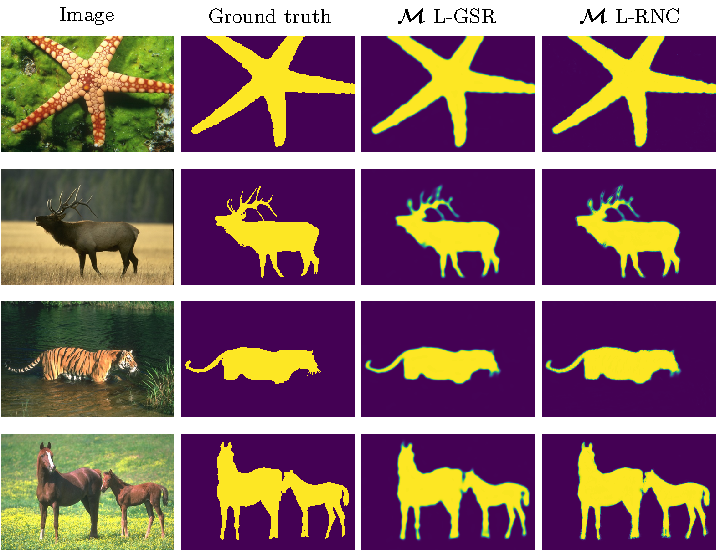
\includegraphics[width=0.8\linewidth]{Figures/segmentation.pdf}
    \end{center}
   \caption[Foreground/background separation with L-GSR and L-RNC]{A colourmap of the output probabilities, $\Mt$, from the L-GSR and L-RNC are shown, along with the original image and the ground truth for the four examples. These were generated with 10\% of the pixels labelled, using an isotropic diffusion filter with $\beta = 50$, and $\gamma = 5 \times 10^{-5}$. For L-RNC, $\lambda$ was set to $10^4$. } 
    \label{fig:foreground_separation}
\end{figure} 

\subsubsection{Assessing accuracy as a function of label percentage}

In the first experiment, we examined the accuracy of each method as a function of the fraction of labelled pixels. \Cref{fig:starfish} provides a visual depiction of the estimated probability tensor $\Mt$ over a range of fractions. As expected, both methods progressively improve as the labelled fraction increases. The L-RNC model appears to outperform the L-GSR, particularly at lower label fractions, likely due to its access to the RGB colour profile in the explanatory tensor $\Xt$. L-GSR, on the other hand, only has access to the lattice graph structure and the location of the labelled pixels. This effect is visible in the first column, where the L-GSR model can only identify the approximate shape of the object, whereas the L-RNC model shows artefacts from the original image, such as the texture of the starfish body. 


\begin{figure}[t] 
    \begin{center}
        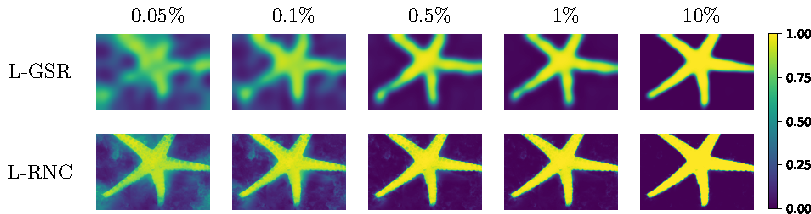
\includegraphics[width=\linewidth]{Figures/starfish.pdf}
    \end{center}
   \caption[Image segmentation output as a function of labelled pixel fraction]{The estimated probability tensor, $\Mt$, output from the L-GSR and L-RNC models, is shown for several fractions of observed data.} 
    \label{fig:starfish}
\end{figure}

To further scrutinise this, we measured each model's accuracy across a range of label fractions for each image. Here, accuracy is gauged by counting the rate of correct predictions for all pixels, by determining whether the probability is less than or greater than 1/2. Simultaneously, we also measured each method's runtime for each label fraction. The results, shown in \cref{fig:fraction_labelled}, reveal both methods steadily improving in accuracy as the label fraction increases. L-RNC generally outperforms L-GSR, especially at lower label percentages, confirming our visual intuition from \cref{fig:starfish}. However, this comes at the cost of a longer runtime, likely due to additional matrix and memory management operations when running the CGM with block matrices. 

It is clear that the runtime of both methods increases as the label fraction grows, consistent with the features of the CGM algorithm, which, as discussed in \cref{sec:GSR_convergence_implications}, is expected to converge quicker when the fraction of missing data is higher. We also observe sporadic spikes in runtime above the general trend, which can likely be attributed to Jax's JIT compiler, which periodically retraces functions to ascertain their impact on inputs of a specific shape and data type \citep{Bradbury2018}.


\begin{figure}[t] 
    \begin{center}
        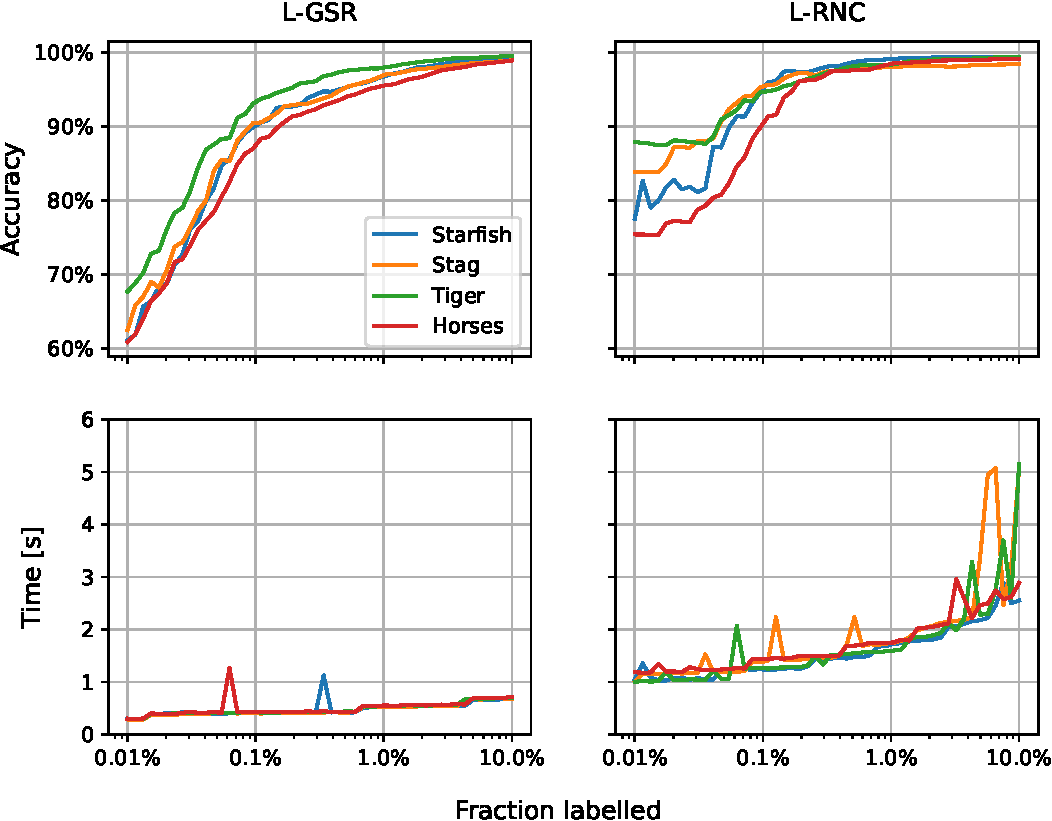
\includegraphics[width=0.9\linewidth]{Figures/fraction_labelled.pdf}
    \end{center}
   \caption[Accuracy of binary L-GSR and L-RNC models as a function of label fraction]{The accuracy on a per-pixel basis is shown for the L-GSR and L-RNC models for each of the four images as a function of the fraction of randomly selected pixels that were labelled} 
    \label{fig:fraction_labelled}
\end{figure}

\subsubsection{Qualitative effects of varying \texorpdfstring{$\gamma$}{gamma} and \texorpdfstring{$\beta$}{beta}}

The second experiment sought to assess the effects on the probability output of the L-GSR and L-RNC algorithms when $\gamma$ and $\beta$ are varied independently. After randomly selecting 0.05\% of the pixels to have their true label revealed, we evaluated the output of the L-GSR and L-RNC algorithms over a range of $\beta$ values while maintaining $\gamma$ fixed at $5 \times 10^{-5}$ and, for L-RNC, $\lambda$ fixed at $100$. Subsequently, we performed the experiment again keeping $\beta$ fixed at 100 and varying $\gamma$. In both cases, an isotropic diffusion filter was used. The results from these experiments are depicted in \cref{fig:starfish2,fig:starfish3}, respectively.

\begin{figure}[t] 
    \begin{center}
        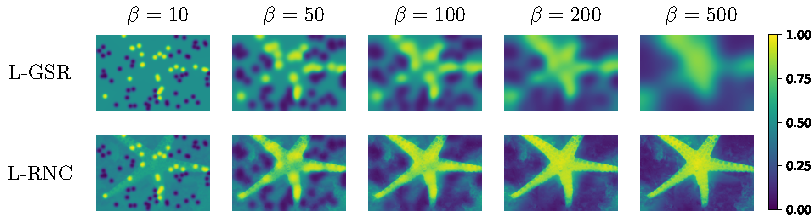
\includegraphics[width=\linewidth]{Figures/starfish2.pdf}
    \end{center}
   \caption[Qualitative effects of varying $\beta$ on the output of the L-GSR and L-RNC algorithms]{A colourmap of the probability output of the L-GSR and L-RNC algorithms are shown for various increasing values of $\beta$. Here, $\gamma$ is set to $5 \times 10^{-5}$ and for L-RNC, $\lambda$ is set to $10^4$. } 
    \label{fig:starfish2}
\end{figure}

\begin{figure}[t] 
    \begin{center}
        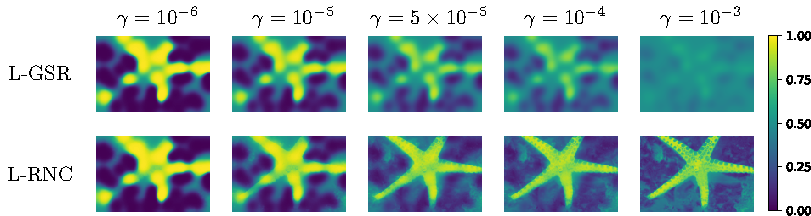
\includegraphics[width=\linewidth]{Figures/starfish3.pdf}
    \end{center}
    \caption[Qualitative effects of varying $\gamma$ on the output of the L-GSR and L-RNC algorithms]{A colourmap of the probability output of the L-GSR and L-RNC algorithms are shown for various increasing values of $\gamma$. Here, $\beta$ is set to $100$ and for L-RNC, $\lambda$ is set to $10^4$.}
    \label{fig:starfish3}
\end{figure}


As seen in \cref{fig:starfish2}, an increase in beta tends to extend the range over which each labelled pixel can influence nearby probability. When $\beta$ is low, at 10, the labelled pixels only affect other pixels in the immediate vicinity, with the probability quickly reverting to 0.5 (i.e. unknown) for more distant unlabelled pixels. As $\beta$ increases, so does this influence range, which is most visible in the L-GSR model where, when $\beta = 500$, the probability prediction becomes quite blurred. Furthermore, these results suggest that increasing $\beta$ assists the L-RNC model in utilising the RGB data, as the outline of the foreground object becomes more defined with the increase in $\beta$.


\Cref{fig:starfish3} illustrates the impact of altering $\gamma$. As visible, a lower $\gamma$ tends to accentuate the transition between class probabilities, with the model yielding probabilities that cluster around zero or one. Interestingly, in this low $\gamma$ region, the graph intercept predominates over the explanatory variables within the L-RNC model. On the other hand, with higher $\gamma$ values, we observe the L-GSR probabilities leaning towards 1/2 across the entire lattice. For the L-RNC model in this scenario, the influence of the graph intercept term wanes, allowing the explanatory variables to take precedence in the prediction process.


\subsection{Multiclass segmentation with hyper-spectral images}
 
In this section, we test the multiclass L-GSR and L-RNC algorithms on a segmentation task using a hyperspectral image of a patch of farmland in North-western Indiana \citep{Baumgardner2015}. The image has been manually segmented into seventeen distinct classes representing different crop types and land uses. The image is $145 \times 145$ pixels in shape, and has 200 channels representing the response over a wavelength range of $0.4-2.5 \times 10^{-6}$m, with some bands covering the region of water absorption removed.  \Cref{fig:hyperspectral} gives an overview of this dataset, with the image on the left an example reading from one of the wavelength channels, and the image on the right a colour representation of the different land types. 

\begin{figure}[t] 
    \begin{center}
        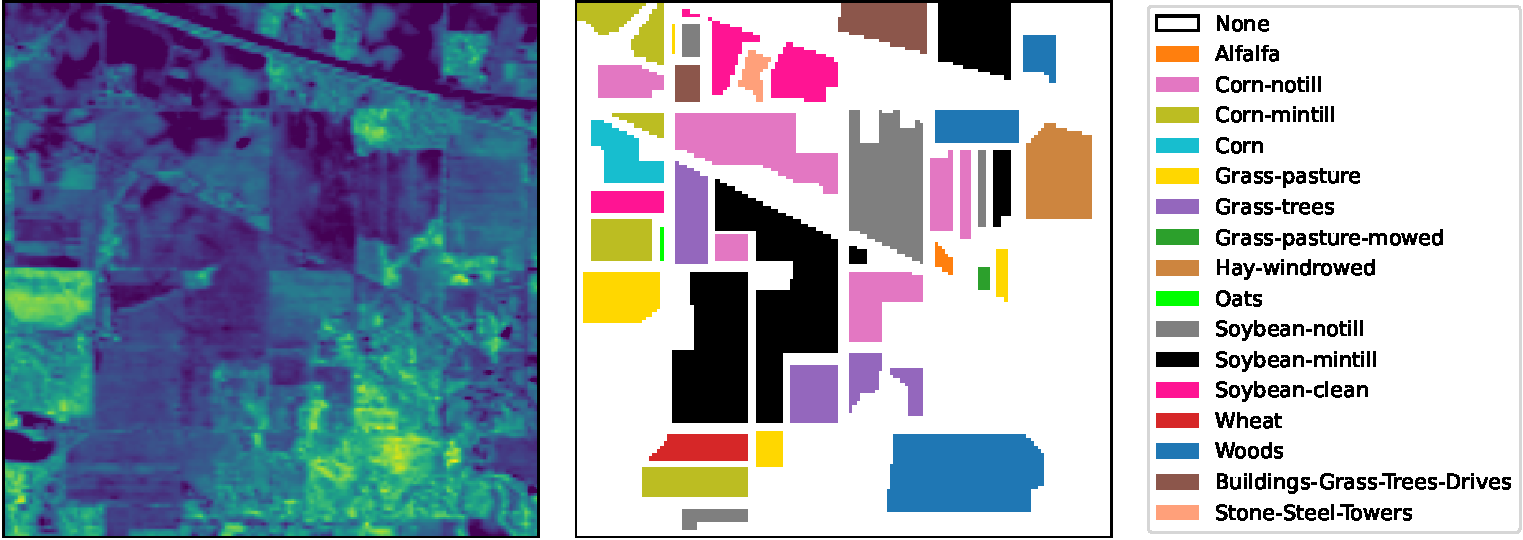
\includegraphics[width=\linewidth]{Figures/hyperspectral.pdf}
    \end{center}
    \caption[A visual overview of the Indian Pines hyperspectral image dataset]{An overview of the Indian Pines hyperspectral image dataset. On the left is an example reading of the intensity response from the channel representing a wavelength of $0.9 \times 10^{-6}$m. On the right is the ground truth for the land use types, along with the associated colour key.}
    \label{fig:hyperspectral}
\end{figure}

In order to verify the algorithms behave as expected, we tested the output when 20\% of the pixels had the correct class labelled. This generated the binary input tensor $\Yt$ of shape $(145, 145, 17)$, with a one-hot encoding along the class dimension, and the sensing tensor $\St$ of shape $(144, 144)$. For the L-RNC algorithm, we allowed access to the pixel data as a tensor of explanatory variables $\Xt$, of shape $(144, 144, 200)$. We then ran the L-GSR and L-RNC algorithms using an isotropic diffusion filter with parameter $\beta = 20$ and set $\gamma = 5 \times 10^{-3}$. For the L-RNC algorithm, we used a regularisation parameter of $\lambda = 100$.  

Both these algorithms produced tensors representing the class probabilities at each pixel in the form of a tensor $\Mt$ of shape $(144, 144, 17)$. From this, we obtained the most likely class by taking the maximum element along the final dimension. The results can be seen in \cref{fig:pines}. The L-GSR model achieved an accuracy of 84\%, and the L-RNC algorithm achieved 89\%. 


\begin{figure}[t] 
    \begin{center}
        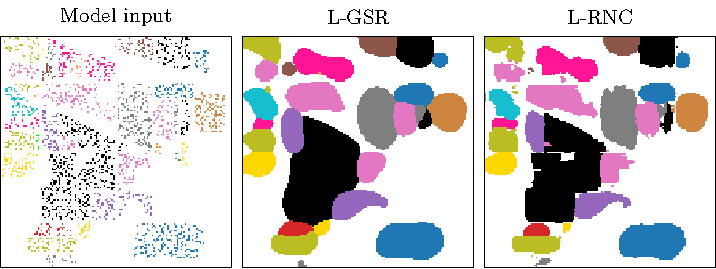
\includegraphics[width=\linewidth]{Figures/pines.pdf}
    \end{center}
    \caption[The predicted class labels from the multiclass L-GSR and L-RNC algorithms as applied to the Indian pines dataset]{A colour representation of the predicted classes from the multiclass L-GSR an L-RNC algorithms as applied to the Indian Pines dataset. On the left, we represent the input $\Yt$ available to the models, which contains 20\% of the labelled pixels randomly selected. }
    \label{fig:pines}
\end{figure}



\section{Discussion}

\subsection{Convergence of the IRLS algorithm}

In general, algorithms based on Newton's method, including Iteratively Reweighted Least Squares (IRLS), frequently encounter convergence difficulties \citep{Kelley2003}. In the course of our experimental work, we encountered two distinct problems, both of which we managed to rectify through relatively straightforward solutions.

Initially, we employed 32-bit floating point numbers for all arrays, with a termination criterion for the IRLS iterations defined as the point at which the absolute change in the target vector or tensor had an average value less than $10^{-6}$. Nevertheless, we often noted an issue where the algorithm failed to converge, with the average change in each element stagnating around the order of $10^{-5}$. To mitigate this issue, we upgraded to 64-bit floating point arrays. Although this change resulted in marginally slower computational speeds and a somewhat larger memory footprint, it effectively addressed the convergence problem.

A second challenge we faced manifested as either divergence or cyclic behaviour, where the target vector would oscillate through a finite series of points without ever achieving convergence. Broadly speaking, we found that these difficulties could be circumvented by selecting a more precise initial value for the iterative process. Our initial strategy was to simply set the initial estimate to a vector of zeros, but this approach led to inconsistent convergence outcomes.

Instead, we found that using an initial estimate derived from the solution to the real-valued GSR/KGR/RNC problem proved to be more effective. To illustrate, for a binary L-GSR problem with inputs $\Yt$, $\St$, $\gamma$, and $\beta$, our initial estimate was the solution to the real-valued GSR problem with inputs $2 \Yt - \St$, $\St$, $\gamma$, and $\beta$. The transformation $\Yt \rightarrow 2 \Yt - \St$ preserves all values equal to one, while all observed values that were zero are converted to negative one, with all unobserved values remaining at zero. This method provided a generally superior initial estimate for the underlying signal, and once implemented, eliminated all previously observed convergence issues. In the case of multiclass problems, we essentially solved the real-valued problem $C$ times, corresponding to each dimension of the class label. This strategy ensured a smoother and more consistent convergence across various hyperparameter settings. 


\subsection{Efficient computation in the multiclass L-RNC algorithm}

It is straightforward to see how the binary L-GSR and L-RNC algorithms can be executed efficiently, using the same ideas used consistently in this thesis. The CGM primarily entails repeated multiplications of the coefficient matrix by an arbitrary vector, while the IRLS algorithm involves repetitive execution of the CGM. In the L-GSR model, the coefficient matrix $\Q$ is constructed solely of diagonal and Kronecker-structured operators, enabling accelerated multiplication onto tensors. This is achieved by efficiently applying \cref{al:GFT_dd}, as elaborated in \cref{sec:GSP_dd}. In the L-RNC scenario, the coefficient matrix $\widetilde{\Q}$ is a block matrix. The blocks aligned along the diagonal consist only of diagonal and Kronecker operators, while the off-diagonal blocks can be directly computed.

As we progress to the multiclass L-GSR algorithm, a complication emerges due to the presence of a non-diagonal, non-Kronecker-structured operator, $\RR_{\muu}$, within the coefficient matrix. Nevertheless, as detailed in \cref{sec:multiclass} and explicitly stated in \cref{eq:R_mu_eff}, the action of $\RR_{\muu}$ on a vector or tensor can be computed efficiently by leveraging its special structure, with a time-complexity of $O(NC)$. 

The multiclass L-RNC, however, presents two additional challenges. First, it becomes necessary to compute the matrix $(\X^\top \otimes \I_C) \RR_{\muu} (\X \otimes \I_C)$, so that it can then be decomposed into $\U_M \LAM_M (\U_M )^\top$. We assume that this decomposition step, which entails solving the eigenvalue problem for a dense symmetric matrix of dimensions $MC \times MC$, is feasible. This assumption is likely reasonable for most problem scenarios. For instance, in our case study involving 200 explanatory variables and 17 classes, the process required the decomposition of a $3400 \times 3400$ matrix. Nevertheless, efficient computation of the matrix $(\X^\top \otimes \I_C) \RR_{\muu} (\X \otimes \I_C)$ is non-trivial. The straightforward strategy of instantiating the $NC \times MC$ matrix $\X \otimes \I_C$ directly, and then sequentially multiplying $\RR_{\muu}$ onto each column demands $C^2$ copies of $\X$, which may be challenging for large problems. In our relatively modest example, this matrix would be of size $(4.2 \times 10^6) \times 3400$, amounting to almost 10GB of 64-bit floating point memory. With a memory complexity of $O(NMC^2)$, this is potentially intractable. 

Fortunately, a more efficient approach is possible. The matrix $(\X^\top \otimes \I_C) \RR_{\muu} (\X \otimes \I_C) \in \R^{MC \times MC}$ can be viewed as a block matrix comprising $M^2$ blocks, each of dimensions $C \times C$. The computation of Block $(i, j)$ can be conducted as follows.

\begin{equation*}
    \text{Block}_{ij} = \text{Block}_{ji} = \Diag{(\X_i \circ \X_j \circ \M)^\top \one_C } - (\X_{i} \circ \M)^\top  (\X_{j} \circ \M)
\end{equation*}

where, in this context, $\X_{i} \in \R^{N \times C}$ is the $i$-th column of $\X$ repeated $C$ times, and $\M$ is $\Mt$ reshaped to have dimensions $(N, C)$. Thus the memory complexity of this approach is reduced to $O(NM + NC)$.  

The second complication that arises is in the computation of the block matrix $\widetilde{\Q}$. Here, the upper right block is given by 

\begin{equation*}
    (\U \D_\Gt \otimes \I_C)^\top \RR_{\muu} (\X \otimes \I_C) \U_M \D_M \in \R^{NC \times MC}
\end{equation*}

and the lower left block is the transpose of this. Again, since this object has $NMC^2$ elements, instantiating it in memory may be problematic. Instead, we can efficiently compute its action on a vector $\ve$ of length $MC$ by taking the following steps.

\begin{enumerate}
    \item $\ve \in \R^{MC} \leftarrow \U_M \D_M \ve \quad$ \textit{(compute this as usual)}
    \item $\ve \in \R^{NC} \leftarrow \vecrm{\X \; \text{reshape}\big(\ve, (M, C)\big)} \quad $ \textit{(compute using the standard row-major vec trick)}
    \item $\ve \in \R^{NC} \leftarrow \RR_{\muu} \ve \quad$ \textit{(compute efficiently using  \cref{eq:R_mu_eff})}
    \item $\ve \in \R^{NC} \leftarrow (\U \D_\Gt \otimes \I_C)^\top \ve \quad$ \textit{(compute efficiently using fast Kronecker product)}
\end{enumerate}

The reverse process, of multiplying the transpose of this block onto a vector of length $NC$ can be achieved by reversing these steps with each operation transposed. In both cases, this reduces the computational and memory footprint substantially.  


\section{Conclusions}

In this chapter, we have considered reconstruction and regression tasks for binary and categorical multiway graph signals. Whilst related tasks have been considered in the machine learning community, in the context of semi-supervised learning \cite{Kondor2002,Zhu2003}, the aims of those models are distinct from our own. In SSL, the graph is usually formed by considering a distance metric in feature space, whereas we take the perspective of GSP, in which the graph is a fundamental structure that preexists, potentially with additional covariates. Although the graph signal processing community has a mature literature on real-valued signals, there have been few papers addressing reconstruction and regression with binary and categorical graph signals. The objective of this chapter has been to present novel classification models applicable to signals existing on general $d$-dimensional Cartesian product graphs, a topic which to the best of our knowledge has not been addressed by the ML or GSP communities. 

In our models, we propose placing a Gaussian graph-spectral prior over a real-valued underlying tensor $\Ft$, which is subsequently transformed via the logistic function to generate class probabilities for each node in the product graph. These probabilities therefore vary smoothly with respect to the topology of the graph, inheriting properties from the graph filter, whilst remaining in the interval $[0, 1]$. 

In particular, we have developed several three novel graph signal processing models by generalising the Graph Signal Reconstruction (GSR), Kernel Graph Regression (KGR), and Regression with Network Cohesion (RNC) models, which were developed earlier in this thesis for real-valued signals, to accommodate binary graph signals. This led to the creation of three ``logistic" models: L-GSR, L-KGR, and L-RNC. Similar to their real-valued counterparts introduced in \cref{chap:nd_gsp}, all three models are devised to handle signals residing on the nodes of general Cartesian product graphs, making them relevant for applications such as network time series modelling. Additionally, we introduced multiclass versions of these three algorithms to manage scenarios where nodes need to be classified into one of several groups or classes. 

These new logistic models required the introduction of a new Iteratively Reweighted Least Squares (IRLS) algorithm to solve for the posterior mean. We discussed the convergence properties of this algorithm in depth, and made proposals for increasing the chances of convergence. In particular, the multiclass models often failed to converge when the initial estimate was a tensor of zeros. However, the chances of success were improved dramatically when we used the solution to the equivalent real-valued problem, with a target tensor of $2\Yt - \St$, as the initial estimate instead. 

